% CVPR 2024 Paper Template; see https://github.com/cvpr-org/author-kit

\documentclass[10pt,twocolumn,letterpaper]{article}

%%%%%%%%% PAPER TYPE  - PLEASE UPDATE FOR FINAL VERSION
\usepackage{cvpr}              % To produce the CAMERA-READY version
% \usepackage[review]{cvpr}      % To produce the REVIEW version
% \usepackage[pagenumbers]{cvpr} % To force page numbers, e.g. for an arXiv version
\usepackage{multirow}
\usepackage[table]{xcolor}
\usepackage{colortbl}
\definecolor{lightred}{rgb}{1, 0.6, 0.6}
\definecolor{lightorange}{rgb}{1, 0.8, 0.5}
\definecolor{lightyellow}{rgb}{1, 1, 0.6}
\usepackage{bm}
\usepackage{rotating} 
\usepackage{stfloats}
\usepackage{subcaption}
\usepackage{graphicx}

% Import additional packages in the preamble file, before hyperref

% It is strongly recommended to use hyperref, especially for the review version.
% hyperref with option pagebackref eases the reviewers' job.
% Please disable hyperref *only* if you encounter grave issues, 
% e.g. with the file validation for the camera-ready version.
%
% If you comment hyperref and then uncomment it, you should delete *.aux before re-running LaTeX.
% (Or just hit 'q' on the first LaTeX run, let it finish, and you should be clear).
\definecolor{cvprblue}{rgb}{0.21,0.49,0.74}
\usepackage[pagebackref,breaklinks,colorlinks,citecolor=cvprblue]{hyperref}

%%%%%%%%% PAPER ID  - PLEASE UPDATE
\def\paperID{*****} % *** Enter the Paper ID here
\def\confName{CVPR}
\def\confYear{2024}

%%%%%%%%% TITLE - PLEASE UPDATE
% \title{HQ-SLAM: Simultaneous Localization and High-quality Photorealistic Mapping for Monocular, Stereo, and RGB-D Cameras }
%\title{Shot-SLAM: Simultaneous Localization and Structure-based Photorealistic Mapping for Monocular, Stereo, and RGB-D Cameras }
\title{\emph{Scaffold}-SLAM: Structured 3D Gaussians for Simultaneous Localization and Photorealistic Mapping }

%%%%%%%%% AUTHORS - PLEASE UPDATE
\author{Tianci Wen \quad 
Zhiang Liu \quad 
Biao Lu \quad
Yongchun Fang \\
Nankai University\\
{\tt\small wentc,liuzhiang,lubiao@mail.nankai.edu.cn, fangyc@nankai.edu.cn}
% For a paper whose authors are all at the same institution,
% omit the following lines up until the closing ``}''.
% Additional authors and addresses can be added with ``\and'',
% just like the second author.
% To save space, use either the email address or home page, not both
}

\begin{document}
\twocolumn[{%
\renewcommand\twocolumn[1][]{#1}%
\maketitle
\begin{center}
  \centering
   %\includegraphics[width=1\linewidth]{fig/fig1.pdf}
        \includegraphics[width=0.16\linewidth]{fig/fig1/tum_rgbd/GS-ICP/01317.png}
        \includegraphics[width=0.16\linewidth]{fig/fig1/tum_rgbd/SplaTAM/01320.png}
        \includegraphics[width=0.16\linewidth]{fig/fig1/tum_rgbd/MonoGS/01317.png}
        \includegraphics[width=0.16\linewidth]{fig/fig1/tum_rgbd/Photo-SLAM/1341848025.834828.png}
        \includegraphics[width=0.16\linewidth]{fig/fig1/tum_rgbd/HQ-SLAM/30000_1296.jpg}
        \includegraphics[width=0.16\linewidth]{fig/fig1/tum_rgbd/GT/30000_1296.jpg}
        \includegraphics[width=0.16\linewidth]{fig/fig1/replica_off3_mono/Photo-SLAM/frame000100.jpg}
        \includegraphics[width=0.16\linewidth]{fig/fig1/replica_off3_mono/HQ-SLAM/30000_100.jpg}
        \includegraphics[width=0.16\linewidth]{fig/fig1/replica_off3_mono/GT/30000_100.jpg}
        \includegraphics[width=0.16\linewidth]{fig/fig1/euroc_stereo/MonoGS/01028.png}
        \includegraphics[width=0.16\linewidth]{fig/fig1/euroc_stereo/HQ-SLAM/30000_1827.jpg}
        \includegraphics[width=0.16\linewidth]{fig/fig1/euroc_stereo/GT/30000_1827.jpg}
   \captionof{figure}{Our method \emph{Scaffold}-SLAM achieves high-quality photorealistic mapping with quality outperforms state-of-the-art methods (GS-ICP SLAM \cite{GS-ICPSLAM2024}, Photo-SLAM \cite{Photo-SLAM2024}, SplaTAM \cite{SplaTAM2024}, MonoGS \cite{MonoGS2024}) across monocular, stereo, and RGB-D cameras. \textbf{Top:} The results are from TUM RGB-D datasets for RGB-D camera. \textbf{Bottom:} The left three images stemming from Replica datasets for monocular camera and the right three from EuRoC MAV datasets for stereo camera. Non-obvious difference in quality highlighted by insets.  % The scene of figure (a)-(f) is fr3/office from TUM RGB-D datasets for RGB-D camera. The scene of figure (g)-(i) is Office3 from Replica datasets for monocular camera.% The scene of figure (j)-(l) is V201\_easy from EuRoC MAV datasets for stereo camera. 
   }   %TODO:添加一行单目双目的结果。
   \label{fig:first_page}
\end{center}%
}]
%\maketitle


\begin{abstract}
We introduce Causal Diffusion as the autoregressive (AR) counterpart of Diffusion models. It is a next-token(s) forecasting framework that is friendly to both discrete and continuous modalities and compatible with existing next-token prediction models like LLaMA and GPT. While recent works attempt to combine diffusion with AR models, we show that introducing sequential factorization to a diffusion model can substantially improve its performance and enables a smooth transition between AR and diffusion generation modes. Hence, we propose \textbf{CausalFusion} - a decoder-only transformer that dual-factorizes data across sequential tokens and diffusion noise levels, leading to state-of-the-art results on the ImageNet generation benchmark while also enjoying the AR advantage of generating an arbitrary number of tokens for in-context reasoning. We further demonstrate CausalFusion's multimodal capabilities through a joint image generation and captioning model, and showcase CausalFusion's ability for zero-shot in-context image manipulations. We hope that this work could provide the community with a fresh perspective on training multimodal models over discrete and continuous data.
\end{abstract}    
\vspace{-10pt}
\section{Introduction}
\label{sec:intro}
Autoregressive (AR) and diffusion models are two powerful paradigms for data distribution modeling. AR models, also known as the next token prediction approach, dominate language modeling and are considered central to the success of large language models (LLMs)~\cite{gpt1,gpt2,gpt3,llama1,llama2,llama3}. On the other hand, diffusion models~\cite{ddpm,dit,adm,edm}, or score-based generative models~\cite{songscore,lipman2023flow}, have emerged as the leading approach for visual generation, driving unprecedented progress in the era of visual content generation~\cite{sora,rombach2022high,li2023scaling}. 

\begin{figure}[t]
    \centering
    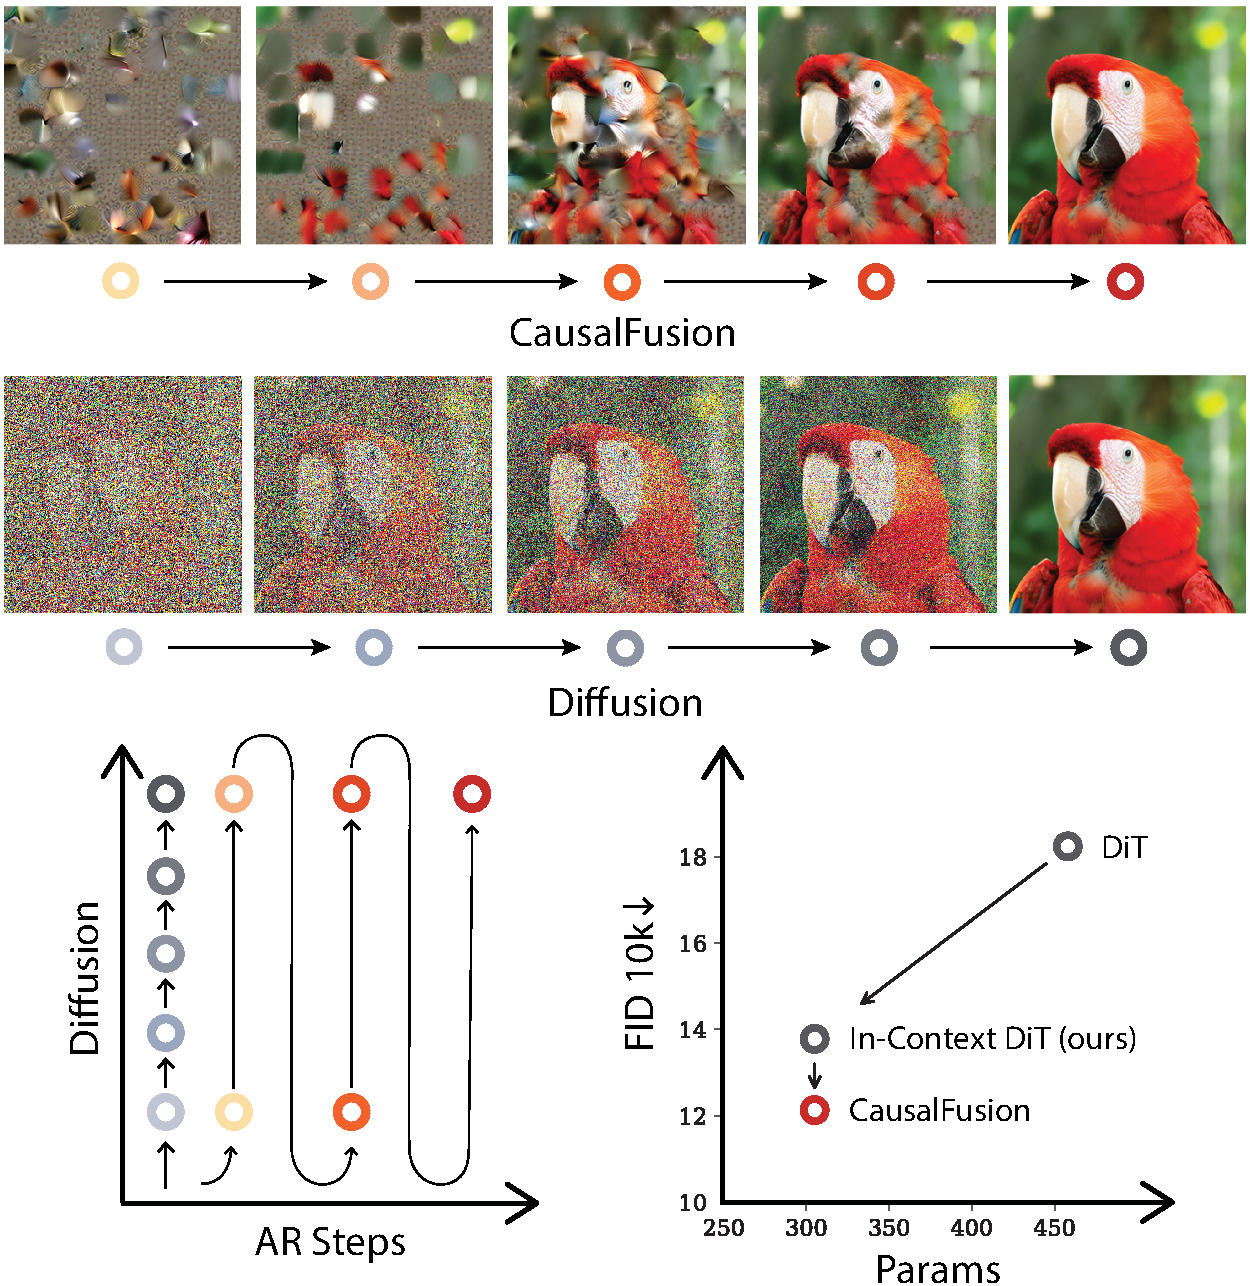
\includegraphics[width=1.0\textwidth,height=1.0\textwidth]{figs/casualfusion-teaser-v6.pdf} 
    \vspace*{-6mm}
    \caption{
    \textbf{Illustration of Dual-Factorization}. The arrow line indicates CausalFusion's generation path, moving from one state to the next by jointly generating along the sequential and noise-level dimension at each step. 
    Compared to DiT, our In-context DiT substantially improves results with fewer parameters. CausalFusion further enhances performance without changing the architecture or parameter count. Results were trained on IN1K for 240 epochs. CausalFusion adopts arbitrary AR steps for image generation, but each step only diffuses partial tokens, resulting in similar (or slightly lower) computational complexity.
    \vspace{-10pt}
    }
    \label{fig:dual-factorization}
\end{figure}


\begin{figure*}[t]
  \centering
  \begin{subfigure}{1.0\linewidth}
    \centering
    \includegraphics[width=\linewidth]{figs/figure2.pdf}
    \caption{Samples generated by CausalFusion-XL/2, ImageNet 512$\times$512, 800 epoch, DDPM 250 steps, CFG=4.0}
  \end{subfigure}
  \begin{subfigure}{1.0\linewidth}
    \centering
    \includegraphics[width=\linewidth]{figs/edit.pdf}
    \caption{\textbf{Zero-shot image editing} results generated by CausalFusion-XL/2, ImageNet 512$\times$512, 800 epoch. We first generate the original image (those on the left), then mask out its centre region, top-half, or bottom-half, and regenerate the image with new class conditions. Details are discussed in Sec \ref{sec:system}.}
  \end{subfigure}
  \caption{\textbf{Visualization results}. All samples are generated by models trained only on \textbf{ImageNet-1K class-conditional generation} task, demonstrating CausalFusion's zero-shot image manipulation ability. See more visualization results in Appendix~\ref{appendix:secD}.
  \vspace{-12pt}
  }
  \vspace{-6pt}
  \label{fig:vis1}
\end{figure*}

The intrinsic distinction between AR and diffusion models lies in their approach to data distribution factorization. AR models treat data as an ordered sequence, factorizing it along the sequential axis, where the probability of each token is conditioned on all preceding tokens. This factorization enables the AR paradigm to generalize effectively and efficiently across arbitrary number of tokens, making it well-suited for long-sequence reasoning and in-context generation. In contrast, diffusion models factorize data along the noise-level axis, where the tokens at each step are a refined (denoised) version of themselves from the previous step. As a result, the diffusion paradigm is generalizable to arbitrary number of data refinement steps, enabling iterative quality improvement with scaled inference compute. While AR and diffusion models each excel within their respective domains, their distinct factorization approaches reveal complementary potential. Although recent studies~\cite{transfusion,monoformer,dart} have attempted to integrate AR and diffusion within a single model, they typically treat these paradigms as separate modes, missing the potential benefits of jointly exploring them within a 2-D factorization plane.

To this end, we introduce \textbf{CausalFusion}, a flexible framework that integrates both sequential and noise-level data factorization to unify their advantages. The degree of factorization along these two axes—namely, the AR step and diffusion step—is adjustable, enabling {CausalFusion} to revert seamlessly to the traditional AR or diffusion paradigms at either extreme. To enhance its generality, CausalFusion is designed to predict \textit{any} number of tokens at \textit{any} AR step, with \textit{any} pre-defined sequence order and \textit{any} level of inference compute, thereby minimizing the inductive biases presented in existing generative models. As shown in Figure~\ref{fig:dual-factorization}, this approach provides a broad spectrum between the AR and diffusion paradigms, allowing smooth interpolation within two endpoints during both training and inference. 
Specifically, we explore CausalFusion in image generation and multimodal generation scenarios, where we observe that the level of training difficulties significantly influences the overall effectiveness of CausalFusion.

\textbf{Difficulties of generative tasks in CausalFusion:} Both AR and diffusion paradigms present unique challenges based on difficulties of their specific generative stages. In diffusion models, the effectiveness of training depends heavily on proper loss weighting across noise levels~\cite{ddpm,minsnr}, as higher noise levels are more difficult and usually provide more valuable signals than lower noise levels. Similarly, AR models are susceptible to error accumulation~\cite{bengio2015scheduled} as early-stage predictions are made with limited visible context, making them more error-prone. Optimizing CausalFusion thus requires balancing across these varying task difficulties to optimize training signal impact and ensure sufficient exploration across the entire factorization plane.

In this paper, we formally examine the difficulties of generative tasks within CausalFusion. We show that, in addition to the noise levels in diffusion and the amount of visible context in AR, the total number of AR steps, which controls the interpolation between AR and diffusion, also plays a critical role in shaping training difficulties. Driven by these factors, we develop a scalable and versatile model based on the CausalFusion framework. Starting from the DiT architecture~\cite{dit}, we gradually convert it into a decoder-only transformer compatible with existing AR models like GPT~\cite{gpt1,gpt2,gpt3} and LLaMA~\cite{llama1,llama2,llama3}. We provide insights on how to appropriately choose the number of AR steps during the training of CausalFusion models, and further introduce loss weighing along both the diffusion and AR axis to balance the impact of different generative stages. As shown in Figure~\ref{fig:dual-factorization} and ~\ref{fig:vis1}, our model achieves state-of-the-art performance on the ImageNet class-conditional generation benchmark, significantly outperforming DiT~\cite{dit} and enabling zero-shot image manipulations due to its AR nature. When pretraining on both text-to-image and image-to-text tasks, our model surpasses forced-fusion frameworks such as TransFusion~\cite{transfusion}, demonstrating the versatility of our CausalFusion framework.


We highlight our main contribution below:
\begin{itemize}
\item  We propose CausalFusion as the AR counterpart to DiT, achieving state-of-the-art results and enabling the unlimited token generation for in-context reasoning.
\item  We systematically study CausalFusion on the dual-factorization plane and identify key factors that improve the effectiveness of CausalFusion models.
\item  Compared with recent studies~\cite{transfusion}, CausalFusion enables a smooth, cohesive integration with language modeling for cross-modal generation and reasoning.
\end{itemize} 

\section{Proposed Method}
\label{sec:method}
%现在我们将展示 \emph{Scaffold}-SLAM,一个具有很高渲染质量的SLAM系统。我们首先简单介绍一下我们方法的骨架:定位与几何建图系统和结构化的3D高斯。随后我们详细描述Appearance-from-Motion Embedding,完成对于场景结构的搭建。最后说明我们用来雕刻环境细节的Frequency-domain Decomposition Pyramid。
In this section, we present details of our \emph{Scaffold}-SLAM. The overview of our SLAM system is summarized in Fig. \ref{fig:diagram}.
%We begin by briefly introducing the framework of our method: the localization and geometric mapping system, alongside structured 3D Gaussians. Next, we provide a detailed description of the two key innovations: Appearance-from-Motion embedding and frequency regularization pyramid.

%-------------------------------------------------------------------------

\subsection{Localization and Geometry Mapping}
%由于传统的基于间接法的SLAM流水线与SfM高度相似,其生成的点云具有很好的几何结构。因此我们跟从传统的基于间接法的SLAM, 我们通过motion-only BA来优化相机位姿。R是相机的朝向,t是相机的位置。通过最小化滑窗内匹配的3-D点与特征点之间的重投影误差来实现:
Since traditional indirect SLAM pipelines are highly similar to SfM, the generated point cloud exhibit robust geometric structure. Thus, we follow the traditional indirect SLAM approach, optimizing the camera orientation $\mathrm{\mathbf{R}}\in SO(3)$ and position $t\in \mathbb{R}^3$ through motion-only bundle adjustment (BA). The camera poses $\{\mathrm{\mathbf{R}},\mathrm{\mathbf{t}}\}$  are optimized by minimizing the reprojection error between the matched 3D points $\mathrm{\mathbf{P}}_i\in \mathbb{R}^3$ and 2D feature points $\mathrm{\mathbf{p}}_i$ within a sliding window:
\begin{align}
\{\mathrm{\mathbf{R}},\mathrm{\mathbf{t}}\}&=  \sum_{i\in\mathcal{X}} \mathop{\mathrm{argmin}}\limits_{\mathrm{\mathbf{R}}_i,\mathrm{\mathbf{t}}_i}  \rho(\|p_j - \pi(\mathrm{\mathbf{R}}_i\mathrm{\mathbf{P}}_j+\mathrm{\mathbf{t}}_i) \|^2_{\Sigma_g}) 
\end{align}
where $\mathcal{X}$ represents the set of all mathches, $\Sigma_g$ denotes the covariance matrix associated with the keypoint's scale, $\pi$ is the projection function, and $\rho$ is the robust Huber cost function. 

We perform a local BA by optimizing a set of covisible keyframes $\mathcal{K}_L$ alone with the set of points ${P}_L$ observed in those keyframes  as follows:
\begin{align}
\{\mathrm{\mathbf{P}}_i,\mathrm{\mathbf{R}}_l,\mathrm{\mathbf{t}}_l\}&= \mathop{\mathrm{argmin}}\limits_{\mathrm{\mathbf{P}}^i,\mathrm{\mathbf{R}}_l,\mathrm{\mathbf{t}}_l} \sum_{k\in \mathcal{K}_L\cup \mathcal{K}_F}  \sum_{j\in \mathcal{X}_k} \rho(E(k,j)) \\
E(k,j) &= \|\mathrm{\mathbf{p}}^j - \pi(\mathrm{\mathbf{R}}_k\mathrm{\mathbf{P}}^j+\mathrm{\mathbf{t}}_k) \|^2_{\Sigma_g}
\end{align}
where $i\in {P}_L$, $l\in \mathcal{K}_L$, $\mathcal{K}_F$ are all other keyframes, and $\mathcal{X}_k$ is the set of matches between keypoints in keyframe $k$ and points in ${P}_L$. 

Global BA is a special case of local BA, where all keyframes and map points are included in the optimization, except the origin keyframe, which is kept fixed to prevent gauge freedom. After performing local or global BA, we can obtain more accurate poses and map point cloud.  %At this stage, we obtain precise camera poses and a structurally sound sparse point cloud $\mathcal{P}$.%至此,我们能获得精确的相机位姿和具有良好结构性的稀疏点云。
%-------------------------------------------------------------------------
\subsection{High-quality Photorealistic Mapping}
% To maximize the utilization of the latent structure within the point cloud, we introduce a region-aware, hierarchical 3D representation, inspired by \textit{Scaffold}-GS. This representation employs fixed anchor points that aim to preserve the environment's structure. Consequently, we incrementally construct a sparse grid of anchor points, initialized by voxelizing the point cloud $\mathcal{P}$ obtained from the geometric mapping. The center coordinates $ \mathrm{\mathbf{x}}_v$ of each voxel serve as anchor points. Each anchor point possesses a context feature $\hat{f}_v \in \mathbb{R}^{32}$, a scale factor $l_v \in \mathbb{R}^{3}$, and a set of $k$ learnable offsets $\mathrm{\mathbf{O}}_v = \{\mathcal{O}_0,\ldots,\mathcal{O}_{k-1} \} \in \mathbb{R}^{k \times 3}$. For each anchor point $\mathrm{\mathbf{x}}_v$ within the view frustum, we can generate $k$ Neural Gaussians and predict their attributes. The positions of $k$ Neural Gaussian are computed using $\mathrm{\mathbf{x}}_v$, the corresponding offset $\mathrm{\mathbf{O}}_v$, and the scale factor $l_v$, as shown below:
% %我们方法表征环境的骨架是一种结构启发的、分层的3D表征形式,它受\textit{Scaffold}-gs启发。我们构造了一个锚点的稀疏网格,它通过体素化ORB-SLAM3几何建图部分得到的点云来初始化。每一个体素的中心坐标x_v即为anchor点。 每个锚点都具有contex特征、尺度因子l_v以及k个可以学习的偏移集合O_v。对于视锥体内每一个anchor点x_v,我们能生成k个 Neural gaussian,并预测他们的attributes。每一个 Neural Gaussian 的位置是通过x_v与相应的偏移量O_v和尺度因子l_v计算的,如下所示:
% \begin{align}
% \{\mu_0,\ldots,\mu_{k-1}\} = \mathrm{\mathbf{x}}_v + \{\mathcal{O}_0,\ldots,\mathcal{O}_{k-1} \} \cdot l_v 
% \end{align}

% The attributes of $k$ Neural Gaussian are directly decoded from the anchor feature $\hat{f}_v$, relative observation distance $\delta_{vc}$, direction $\vec{\mathrm{\mathbf{d}}}_{vc}$, or appearance encoding $\bm{\ell}^a_i$. Each attribute is decoded using individual MLPs, denoted as \(M_\alpha\), \(M_c\), \(M_q\), and \(M_s\), respectively. For example, the color of Neural Gaussians is obtained as follows:
% %Neural gaussian的attributes是直接根据anchor特征、相对观测距离和方向或者外观编码解码得到的。每一个attribute都采用单独的MLP作为解码器,即M_\alpha, M_c, M_q 和M_s。例如Neural gaussian的颜色是这么得到的:
% \begin{align}
% \{c_0,\dots,c_{k-1}\} = M_C(\hat{f}_v,\ \delta_{vc},\ \vec{\mathrm{\mathbf{d}}}_{vc},\ \bm{\ell}^{(a)}_{\mathrm{\mathbf{R}}_i,\ \mathrm{\mathbf{t}}_i})
% \end{align}
% %他们的不透明度、四元数、尺度通过类似的方式得到,不过只有颜色包含外观编码信息。更多的细节,请参阅\textit{Scaffold}-gs。
% where $\delta_{vc} = \| x_v-x_c\|_2,\  \vec{\mathrm{\mathbf{d}}}_{vc} = (x_v-x_c) / \| x_v-x_c\|_2$. Their opacity $\{\alpha_i\}$, quaternion $\{q_i\}$, and scale $\{s_i\}$ are similarly obtained. Only the color $\{c_i\}$ incorporates appearance embedding. For further details, please refer to \textit{Scaffold}-gs.
% %在得到视锥体内每一个Neural Gaussian $G(x)$的attributes之后,将其投影至图像平面得到2D Gaussian。跟从3DGS, 一个基于块的渲染器来排序2DGaussians,并采用\alpha - blending来完成渲染:
% After obtaining the attributes of each Neural Gaussian $G(x)$ within the view frustum, it is projected onto the image plane to form a 2D Gaussian $G^\prime_i(x^\prime)$. Following 3DGS, a tile-based rasterizer is used to sort the 2D Gaussians, and $\alpha-$blending is employed to complete the rendering:
% \begin{align}
%     C(x^\prime) = \sum_{i\in N} c_i \delta_i \prod_{j=1}^{i-1}(1 - \delta_j), \quad \delta_i = \alpha_i G^\prime_i(x^\prime)
%   \label{eq:rendering}    
% \end{align}
% where $x^\prime$ is the pixel position and N is the number of corresponding 2D Gaussians for each pixel.

%与Photo-SLAM不一样。受Scaffold-GS启发,在本文中,我们选择了一种结构化的3D高斯作为我们场景表征的基础。因为它具备更良好的扩展性,并且能更好地保留点云的几何结构,从而保证对于不同相机类型的高质量真实感建图。与3DGS一样,它的渲染过程如下:
Following 3DGS, our rendering process is as follows:
\begin{align}
    C(\mathrm{\mathbf{R}},\mathrm{\mathbf{t}}) = \sum_{i\in N} c_i \delta_i \prod_{j=1}^{i-1}(1 - \delta_j)
  \label{eq:rendering}    
\end{align}
where $N$ is the number of ordered 2D Gaussians overlapping the pixel, $\delta_i = \alpha_i \cdot \mathcal{G}(\mathrm{\mathbf{R}},\mathrm{\mathbf{t}}, \mathrm{\mathbf{P}}_i, \mathrm{\mathbf{q}}_i, \mathrm{\mathbf{s}}_i)$, and $\mathcal{G}$ denotes splatting process of 3DGS \cite{3DGS2023}.  The parameters of 3D Gaussians include color $c$, position $\mathrm{\mathbf{P}}$, scaling matrix $\mathrm{\mathbf{s}}$, rotation matrix $\mathrm{\mathbf{q}}$, and opacity $\alpha$. Inspired by \cite{Scaffold-GS2024}, we incrementally construct a sparse grid of anchor points, initialized by voxelizing the point cloud obtained from the geometric mapping. Each anchor point distributes $k$ 3D Gaussians, the color of which is obtained as follows:
\begin{align}
\{c_0,\dots,c_{k-1}\} = M_c(\hat{f}_v,\ \delta_{vc},\ \vec{\mathrm{\mathbf{d}}}_{vc},\ \bm{\ell}^{(a)}_{\mathrm{\mathbf{R}},\ \mathrm{\mathbf{t}}})
\end{align}
where $\delta_{vc},\  \vec{\mathrm{\mathbf{d}}}_{vc}$ are relative distance and viewing direction of the anchor point, $\hat{f}_v$ is a local context feature, and $M_c$ is a individual multi-layer perceptron (MLP). $\alpha$, $\mathrm{\mathbf{q}}$, and $\mathrm{\mathbf{s}}$ are similarly obtained by individual MLPs, denoted as \(M_\alpha\), \(M_q\), and \(M_s\), respectively. Only the color $c$ incorporates Appearance-from-Motion embedding $\bm{\ell}^{(a)}_{\mathrm{\mathbf{R}},\ \mathrm{\mathbf{t}}}$. %Since this representation effectively leverages the scene structure, and the point clouds generated by traditional indirect visual SLAM also exhibit strong structural coherence, we believe this combination can push the upper limits of photorealistic mapping quality.
%其中Ci代表3D高斯的颜色。与3DGS不同,颜色按照这样得到 For further details, please refer to \cite{Scaffold-GS2024}.



\subsubsection{Appearance-from-Motion Embedding}
%Appearance Embedding是在NerF和3DGS中均被使用的技术。它最早来自于一种生成式网络 Generative Latent Optimization,NeRF-W中首次将这个技术引入神经渲染,它通过学习所有图片之间的共享外观表征来建模每张图像的光照和环境变化。\textit{Scaffold}-GS也将这个技术引入了显示渲染,提升算法的渲染质量。这种 Embedding的输入为每张图像的index,它采用了一个Embedding layer将外观变化建模到一个低维的latent space。 但是,NeRF-W不仅仅在训练集训练 appearance Embedding。对于测试集的每张图片,它采用左半张图片训练appearance Embedding去学习这张图片的外观变化,然后评估指标采用右半张图片。对于NVS,他们任务包含数百个视角,有约20%左右为测试集,这种操作的代价可以接受。但是SLAM的数据集通常包含数千张图片,有约80%为测试集,这种代价太大不能接受。\textit{Scaffold}-GS为了避免在测试集上训练appearance Embedding,他们在测试集上随机选择一个训练集的index作为输入,这种做法对于SLAM这种测试集占比巨大的任务来说在测试集上的效果会很差。
%为了解决这个问题,我们不再采用每个图像的index作为appearance Embedding,我们采用每张图像对应的估计的相机位姿作为输入。采用这种方式背后的依据是,由于我们SLAM系统所有位姿采用了全局BA来优化,所有估计的位姿服从同一个概率分布(MAP),因此我们可以采用一个网络学习图像外观与位姿潜在概率分布之间的关系,从而实现对于没有训练的测试集进行推理。我们称这种方法为Appearance-from-Motion Embedding,实验结果证明两它的有效性,如图2所示,最重要的无需在测试集上训练。在实现中,我们采用一个小的MLP来学习每个图像外观变化和其相机位姿的潜在关系,如下所示
To handle photometric variations, appearance embedding is a proven effective technique. It originates from a generative network called Generative Latent Optimization \cite{GLO2019}. NeRF-W \cite{NeRF-W2021} is the first to introduce this technique into neural rendering. By learning a shared appearance representation across all images, it models per-image photometric and environmental variations in a low-dimensional latent space. Each image is assigned a corresponding appearance embedding real-valued vector $\bm{\ell}^{(a)}_i$ of length $n^{(a)}$ which takes the index $i$ of each image as input.  \textit{Scaffold}-GS \cite{Scaffold-GS2024} also incorporates this technique to enhance the rendering quality. However, in NeRF-W, the embedding $\bm{\ell}^{(a)}_i$ is not only trained on the training set. When evaluating error metrics on test-set, NeRF-W trains $\bm{\ell}^{(a)}_i$ using the left half of the groundtruth image to match the appearance and evaluates metrics on the right half. In the novel view synthesis dataset, there are typically hundreds of views, with approximately 20\% allocated to the test-set, making the computational cost of this approach acceptable. However, in SLAM datasets, which contain thousands of images with around 80\% being test-set, this cost becomes prohibitive. \textit{Scaffold}-GS addresses this by randomly selecting a training image index as input for test images. Nevertheless, this approach performs poorly for tasks like SLAM, where the test-set is large. Because the trained views are too sparse relative to the novel views, making it difficult to predict the appearance of novel views.

\begin{figure}[t]
	\centering
    \begin{subfigure}[ht]{0.495\linewidth}
        \includegraphics[width=1\linewidth]{fig/fig_AE/base+FRP/30000_10_mark.jpg}
        \caption{w/o AfME}
    \end{subfigure}    \hspace{-1.5mm}
    \begin{subfigure}[ht]{0.495\linewidth}
        \includegraphics[width=1\linewidth]{fig/fig_AE/ours/30000_10_mark.jpg}
        \caption{ \emph{Scaffold}-SLAM}
    \end{subfigure}    
	\caption{Illustration of the appearance variations  modeled by Appearance-from-Motion embedding. All images are rendered from novel views with significant lighting changes.}
	\label{fig:result_include1}
\end{figure}
% \begin{figure}[t]
% 	\centering
%     % \begin{subfigure}[ht]{0.16\linewidth}
%     %     \includegraphics[width=1\linewidth]{fig/fig3_methods/1/train/30000_602.jpg}
%     % \end{subfigure}
%     %  \hspace{-1.5mm}
%     \begin{subfigure}[ht]{0.16\linewidth}
%         \includegraphics[width=1\linewidth]{fig/fig3_methods/1/test/30000_615.jpg}
%     \end{subfigure}     \hspace{-1.5mm}
%     \begin{subfigure}[ht]{0.16\linewidth}
%         \includegraphics[width=1\linewidth]{fig/fig3_methods/1/test/30000_640.jpg}
%     \end{subfigure}    \hspace{-1.5mm}
%     \begin{subfigure}[ht]{0.16\linewidth}
%         \includegraphics[width=1\linewidth]{fig/fig3_methods/1/test/30000_682.jpg}
%     \end{subfigure}    \hspace{-1.5mm}
%     \begin{subfigure}[ht]{0.16\linewidth}
%         \includegraphics[width=1\linewidth]{fig/fig3_methods/1/test/30000_710.jpg}
%     \end{subfigure}    \hspace{-1.5mm}
%     \begin{subfigure}[ht]{0.16\linewidth}
%         \includegraphics[width=1\linewidth]{fig/fig3_methods/1/test/30000_745.jpg}
%     \end{subfigure}    \hspace{-1.5mm}
%     \begin{subfigure}[ht]{0.16\linewidth}
%         \includegraphics[width=1\linewidth]{fig/fig3_methods/1/test/30000_781.jpg}
%     \end{subfigure}    
%     %\hspace{-1.5mm}
%     % \begin{subfigure}[ht]{0.16\linewidth}
%     %     \includegraphics[width=1\linewidth]{fig/fig3_methods/1/train/30000_815.jpg}
%     % \end{subfigure}

%     % \begin{subfigure}[ht]{0.16\linewidth}
%     %     \includegraphics[width=1\linewidth]{fig/fig3_methods/2/trian/30000_1376.jpg}
%     % \end{subfigure}    \hspace{-1.5mm}
%     \begin{subfigure}[ht]{0.16\linewidth}
%         \includegraphics[width=1\linewidth]{fig/fig3_methods/2/test/30000_1405.jpg}
%     \end{subfigure}    \hspace{-1.5mm}
%     \begin{subfigure}[ht]{0.16\linewidth}
%         \includegraphics[width=1\linewidth]{fig/fig3_methods/2/test/30000_1480.jpg}
%     \end{subfigure}    \hspace{-1.5mm}
%     \begin{subfigure}[ht]{0.16\linewidth}
%         \includegraphics[width=1\linewidth]{fig/fig3_methods/2/test/30000_1570.jpg}
%     \end{subfigure}    \hspace{-1.5mm}
%     \begin{subfigure}[ht]{0.16\linewidth}
%         \includegraphics[width=1\linewidth]{fig/fig3_methods/2/test/30000_1600.jpg}
%     \end{subfigure}    \hspace{-1.5mm}
%     \begin{subfigure}[ht]{0.16\linewidth}
%         \includegraphics[width=1\linewidth]{fig/fig3_methods/2/test/30000_1630.jpg}
%     \end{subfigure}    \hspace{-1.5mm}
%     \begin{subfigure}[ht]{0.16\linewidth}
%         \includegraphics[width=1\linewidth]{fig/fig3_methods/2/test/30000_1645.jpg}
%     \end{subfigure}    
%     %\hspace{-1.5mm}
%     % \begin{subfigure}[ht]{0.16\linewidth}
%     %     \includegraphics[width=1\linewidth]{fig/fig3_methods/2/trian/30000_1676.jpg}
%     % \end{subfigure}

%     % \begin{subfigure}[ht]{0.16\linewidth}
%     %     \includegraphics[width=1\linewidth]{fig/fig3_methods/3/Train/30000_0.jpg}
%     %     % \caption{TV}
%     % \end{subfigure}    \hspace{-1.5mm}
%     \begin{subfigure}[ht]{0.16\linewidth}
%         \includegraphics[width=1\linewidth]{fig/fig3_methods/3/Test/30000_56.jpg}
%         % \caption{NV}
%     \end{subfigure}    \hspace{-1.5mm}
%     \begin{subfigure}[ht]{0.16\linewidth}
%         \includegraphics[width=1\linewidth]{fig/fig3_methods/3/Test/30000_89.jpg}
%         % \caption{NV}
%     \end{subfigure}    \hspace{-1.5mm}
%     \begin{subfigure}[ht]{0.16\linewidth}
%         \includegraphics[width=1\linewidth]{fig/fig3_methods/3/Test/30000_126.jpg}
%         % \caption{NV}
%     \end{subfigure}    \hspace{-1.5mm}
%     \begin{subfigure}[ht]{0.16\linewidth}
%         \includegraphics[width=1\linewidth]{fig/fig3_methods/3/Test/30000_166.jpg}
%         % \caption{NV}
%     \end{subfigure}    \hspace{-1.5mm}
%     \begin{subfigure}[ht]{0.16\linewidth}
%         \includegraphics[width=1\linewidth]{fig/fig3_methods/3/Test/30000_203.jpg}
%         % \caption{NV}
%     \end{subfigure}    \hspace{-1.5mm}
%     \begin{subfigure}[ht]{0.16\linewidth}
%         \includegraphics[width=1\linewidth]{fig/fig3_methods/3/Test/30000_228.jpg}
%         % \caption{NV}
%     \end{subfigure}    
%     %\hspace{-1.5mm}
%     % \begin{subfigure}[ht]{0.16\linewidth}
%     %     \includegraphics[width=1\linewidth]{fig/fig3_methods/3/Train/30000_257.jpg}
%     %     % \caption{TV}
%     % \end{subfigure}
% 	\caption{Illustration of the appearance variations  modeled by Appearance-from-Motion embedding. All images are rendered from novel views with significant lighting changes.}
% 	\label{fig:result_include1}
% \end{figure}

Fortunately, our focus is on photorealistic mapping of SLAM. It naturally follows that we would use the estimated camera pose corresponding to each training image as the input for appearance embedding, rather than the image index. Our insight is that the camera poses optimized through global bundle adjustment conform to the same maximum a posteriori (MAP) probability distribution. Moreover, each image corresponding to a unique camera pose, which shares analogous properties with the camera indices. Therefore, we can train a network to learn a shared appearance representation across all training camera poses, capturing the underlying probabilistic distribution of these poses. Since the camera poses of test-set also belong to this distribution, the network can predict the appearance for the novel views. We refer to this method as Appearance-from-Motion embedding. We employ a tiny MLP to model the appearance variation of each image based on its camera pose in a low-dimensional latent space, as shown below:
\begin{align}
    \bm{\ell}^{(a)}_{\mathrm{\mathbf{R}},\ \mathrm{\mathbf{t}}} &= \mathrm{MLP}_{\Theta_a}(\mathrm{\mathbf{R}},\ \mathrm{\mathbf{t}})
  \label{eq:embedding}    
\end{align}
Subsequently, this Appearance-from-Motion embedding $\bm{\ell}^{(a)}_{\mathrm{\mathbf{R}},\ \mathrm{\mathbf{t}}}$ is fed into the color decoder $M_c$, allowing all pixels in an image to share the same appearance representation. Ultimately, the appearance of all images is modeled within a continuous latent space, as illustrated in the Fig. \ref{fig:result_include1}. We emphasize once again that our Appearance-from-Motion embedding does not require training on the test-set.
%-------------------------------------------------------------------------
\subsubsection{  Frequency regularization Pyramid }
%为了提升方法的真实感建图质量,另外一个需要解决的问题是渲染图像在场景中的高频细节处表现很差。例如中物体的边缘以及纹理复杂的区域。 FreGS首先采用了一种结合频率正则与频率退火的策略。他们将频域中的高频和低频分解出来,使得高斯能更加高效地稠密化。然而这种策略使得模型只能学到较为单一的细节。
%为了充分利用各种merits,我们提出了 hierarchical high-frequency refinement,一种新的频率正则技术。我们进一步引入了多尺度的信息,使得模型能学习不同层次的细节。具体来说,我们通过多种尺度的渲染图像与相应真值之间频谱的差异构造了一个损失,用来监督anchor的生长。本文只采用高频频率来监督,因为低频频率一般用于鼓励模型学习环境中的结构。这种结构已经被anchor点良好地利用了。

%为了充分利用更多层次的细节,我们提出了 Frequency Regulariztion Pyramid,一种新的频率正则技术。为了构造不同尺度的图像,我们对真值和渲染图像通过bilinear插值对图像进行平滑地缩小。在训练过程中,我们将同时使用多尺度图像的频率来监督模型的训练。具体来说,对于所有尺度的渲染图像和真值图像,我们首先对其应用2维的快速傅里叶变换,得到图像的频谱。随后我们对于该频谱应用高通滤波器来提取图像中的高频区域。然后我们根据多种尺度的渲染图像与相应真值图像之间高频频谱的差异构造了一个损失,如下所示。

%与FreGS不同,我们没有采用低频频率来监督我们的模型。因为低频频率一般用于鼓励模型学习环境中的结构,然而我们的几何建图部分生成了良好环境结构的点云来初始化我们的高斯。我们采用了一种退火策略来指导频率金字塔的监督。由于SLAM的场景是增量式构建的,其环境结构需要一定的时间才能够稳定,因此我们选择在经过一定量的迭代次数后才添加多尺度频率监督。另外,在优化的末期,环境的结构和细节都相当稳定之后,我们将会停止频率监督。
%多加点描述,关于退火、滤波等等;前面embedding添加map的公式
To improve the quality of the photorealistic mapping, another challenge is the poor performance of the rendered images in capturing high-frequency details, particularly around object edges and regions with complex textures. Some prior works offer potential solutions: HF-NeuS \cite{HF-NeuS2022} employs a coarse-to-fine strategy to decompose SDF into base and displacement functions, gradually enhancing high-frequency details. AligNeRF \cite{AligNeRF2023} improves upon the perceptual loss proposed by Johnson \cite{Johnson} to enhance high-frequency rendering details. FreGS \cite{FreGS2024} introduces a strategy combining frequency regularization with frequency annealing. They decompose the high and low frequencies in the frequency domain, allowing the Gaussians to densify more efficiently. We find that this frequency regularization approach can control the growth of anchor points. However, its limitation is that the model can only learn high-frequency details through single-scale features.

To fully leverage multiple levels of detail, we propose a novel frequency regularization technique called the frequency regularization pyramid. To construct images at different scales, we apply bilinear interpolation to smoothly downsample both the ground truth and rendered images. During training, we supervise the model with the frequency from multi-scale images. Specifically, Let $s \in \mathcal{S} = \{s_0, s_1, \ldots, s_n\}$ denotes the scale of an image. For all scales of both the rendered images $I_r^{s}$ and ground truth images $I_g^{s}$, we first apply a 2D Fast Fourier Transform (FFT) to obtain the frequency spectra $\mathcal{F}(I_r^{s})(u, v), \mathcal{F}(I_g^{s})(u, v)$. We then use a high-pass filter $H_f(u, v)$ on these spectra to extract the high-frequency $F_{r, f}^{s}(u, v), F_{g, f}^{s}(u, v)$. The loss $\mathcal{L}_{\text{vol}}$ is computed based on the difference in high-frequency spectra between the rendered and ground truth images across different scales, as shown below:
\begin{align}
\mathcal{L}_{f} &=\lambda_h \sum_{s \in \mathcal{S}} \frac{1}{N} \sum_{u, v} \left| F_{r, h}^{s}(u, v) - F_{g, j}^{s}(u, v) \right|  \\
F_{i, f}^{s}(u, v) &= H_f(u, v) \cdot \mathcal{F}(I_i^{s})(u, v), f\in \{h, l\},\ i\in \{r, g\} \nonumber
\end{align} \\
where $N =HW$ denotes the size of the image. Unlike FreGS, we do not use low-frequency information to supervise our model. This is because low-frequency components are typically used to encourage the model to learn the overall structure of the environment. However, in our case, the geometric mapping process already generates a well-structured point cloud that is used to initialize the Gaussians. Moreover, we employ an annealing strategy to guide the supervision of the frequency regularization pyramid. Since the SLAM system incrementally builds the scene and requires time for the environment structure to stabilize, we introduce frequency regularization pyramid only after a certain number of iterations $T_s$. Furthermore, as the scene's structure and details become stable toward the end of optimization, we stop applying frequency supervision after $T_e$ iterations.

\subsubsection{Optimization}
%最终,模型中可学习的参数、预测高斯颜色、尺度、旋转、和不透明度的MLP以及Appearance-from-Motion Embedding的MLP的优化,通过对渲染图像与真值图像之间的L1损失、SSIM项、频率正则以及体积正则进行最小化:

Finally, the optimization of the learnable parameters in the model, the MLP that predicts parameters of 3D Gaussians, and the MLP for Appearance-from-Motion embedding are achieved by minimizing the L1 loss $\mathcal{L}_1$, SSIM term, frequency regularization $\mathcal{L}_{f}$, and volume regularization $\mathcal{L}_{\text{vol}}$ between the rendered images and the ground truth images, denoted as
\begin{align}
\mathcal{L} = (1-\lambda)\mathcal{L}_1 +  \lambda(1-\mathcal{L}_{\text{SSIM}}) +\lambda_{\text{vol}}\mathcal{L}_{\text{vol}} + \lambda_{f} \mathcal{L}_{f}
\end{align}
where 
\begin{align}
\mathcal{L}_{\text{vol}} =\sum_{i=1}^{N_{ng}}\text{Prod}(s_i)
\end{align}
Here, $\text{Prod}(\cdot)$ denotes product of the values of a vector and $N_{ng}$ presents the number of 3D Gaussians.
% \begin{align}
% F_{i, f}^{s}(u, v) &= H_f(u, v) \cdot \mathcal{F}(I_i^{s})(u, v)
% \end{align}
% where $\quad f\in \{h, l\},\ i\in \{r, g\}$

% \begin{align}
% \mathcal{L}_{f}^{s} &= \frac{1}{N} \sum_{u, v} \left| F_{r, f}^{s}(u, v) - F_{g, f}^{s}(u, v) \right| \\
% \mathcal{L}_{\text{freq}} &= \sum_{s \in \{s_0, s_1, \ldots, s_n\}} \left( \lambda_l \mathcal{L}_{l}^{s} + \lambda_h \mathcal{L}_{h}^{s} \right)
% \end{align}
% where $N =HW$,

% \begin{align}
% \mathcal{L}_{\text{freq}} = (1-\lambda)\mathcal{L}_1 +  \lambda\mathcal{L}_{\text{D-SSIM}} +\lambda_{\text{vol}}\mathcal{L}_{\text{vol}} + \mathcal{L}_{\text{freq}}
% \end{align}
%-------------------------------------------------------------------------
% \begin{table*}
% \footnotesize
% %\small
% %\normalsize
% \setlength\tabcolsep{5pt}
% %\renewcommand{\arraystretch}{0.8}
%   \centering
%   \begin{tabular}{l|c|ccccccccc|cccc} %{|p{3cm}|c|c|}
%     \toprule \noalign{\vskip -2pt}
%     \multicolumn{2}{c|}{Datasets}  & \multicolumn{9}{c|}{Replica } & \multicolumn{4}{c}{TUM RGB-D}\\ 
%     \hline 
%     \noalign{\vskip 0.7pt}
%     Method & Metric & R0 & R1 & R2 & Of0 & Of1 & Of2 & Of3 & Of4 & Avg. & fr1/d & fr2/x & fr3/o & Avg.\\
%     \hline %\midrule[0.1pt] %\hline
%     \noalign{\vskip 0.4pt}
%     \multirow{3}{*}{MonoGS} &  PSNR$\uparrow$   & 34.29 & 35.77 & 36.79 & 40.87 & 40.73 & 35.22 & 35.89 & 34.98 & 36.82 &23.59& 24.46 & 24.29 & 24.11\\
%     &SSIM$\uparrow$   & 0.953 & 0.957 & 0.965 & 0.979 & 0.977 & 0.961 & 0.962 & 0.955 & 0.964 &0.783 & 0.789 & 0.829 & 0.800\\
%     &LPIPS$\downarrow$  & 0.071 & 0.078 & 0.074 & 0.048 & 0.052 & 0.074 & 0.061 & 0.092 & 0.069 &0.244 & 0.227 & 0.223 & 0.231\\
%     \hline %\midrule[0.1pt] %\hline
%     \noalign{\vskip 0.4pt} % 21.2469326	0.740986669	0.207413478
%     \multirow{3}{*}{Photo-SLAM} &  PSNR$\uparrow$   & 32.09 & 34.15 & 35.91 & 38.70 & 39.53 & 33.13 & 34.15 & 36.35 & 35.50 &20.58 & 22.12 &21.05 &21.25\\
%     &SSIM$\uparrow$   & 0.920 & 0.941 & 0.959 & 0.967 & 0.964 & 0.943 & 0.943 & 0.956 & 0.949 &0.729 & 0.764 &0.730 &0.741\\
%     &LPIPS$\downarrow$  & 0.069 & 0.055 & 0.041 & 0.048 & 0.045 & 0.075 & 0.064 & 0.053 & 0.056 &0.252 & 0.171 &0.200 &0.207\\
%     \hline %\midrule[0.1pt] %\hline
%     \noalign{\vskip 0.4pt}


%     \multirow{3}{*}{Photo-SLAM-30K} &  PSNR$\uparrow$   & 31.41 & 35.84 & 38.41 & 40.44 & 41.06 & 34.56 & 35.43 & 38.36 & 36.94  & 21.78 & 21.57 & 21.84 & 21.73\\
%     &SSIM$\uparrow$   & 0.873 & 0.955 & 0.971 & 0.975 & 0.972 & 0.952 & 0.954 & 0.967 & 0.952 & 0.766 & 0.755 & 0.751 & 0.757\\
%     &LPIPS$\downarrow$  & 0.046 & 0.036 & 0.026 & 0.033 & 0.033 & 0.059 & 0.049 & 0.036 & 0.040 &0.212& 0.182 &0.165 & 0.186\\
%     \hline %\midrule[0.1pt] %\hline
%     \noalign{\vskip 0.4pt}
%     \multirow{3}{*}{RTG-SLAM} &  PSNR$\uparrow$   & 28.49 & 31.27 & 32.96 & 37.32 & 36.12 & 31.14 & 31.19 & 33.81 & 32.79 &13.62 & 17.08 & 18.70 & 16.47\\
%     &SSIM$\uparrow$   & 0.834 & 0.902 & 0.927 & 0.957 & 0.943 & 0.923 & 0.918 & 0.937 & 0.918 &0.501 & 0.573 & 0.648 & 0.574\\
%     &LPIPS$\downarrow$  & 0.152 & 0.169 & 0.162 & 0.084 & 0.103 & 0.145 & 0.139 & 0.165 & 0.164 &0.557 & 0.403 & 0.422 & 0.461\\
%     \hline %\midrule[0.1pt] %\hline
%     \noalign{\vskip 0.4pt}
%     \multirow{3}{*}{GS-SLAM} &  PSNR$\uparrow$   & 31.56 & 32.86 &32.59 &38.70 &41.17 &32.36 &32.03 &32.92 &34.27 &- & - &- &-\\
%     &SSIM$\uparrow$   & 0.968 & 0.973 & 0.971 & 0.986 & 0.993 & 0.978 & 0.970 & 0.968 & 0.975 &- & - &- &-\\
%     &LPIPS$\downarrow$  & 0.094 & 0.075 & 0.093 & 0.050 & 0.033 & 0.094 & 0.160 & 0.162 & 0.082 &- & - &- &-\\
%     \hline %\midrule[0.1pt] %\hline
%     \noalign{\vskip 0.4pt}
%     \multirow{3}{*}{SplaTAM} &  PSNR$\uparrow$   & 32.48 & 33.50 & 35.11 & 38.22 & 38.91 & 31.86 & 30.05 & 31.53 & 33.96 &22.88 & 26.52 &21.38 &23.60\\
%     &SSIM$\uparrow$   & 0.975 & 0.968 & 0.983 & 0.983 & 0.982 & 0.966 & 0.952 & 0.946 & 0.969 & 0.910 & 0.955 &0.865 &0.910\\
%     &LPIPS$\downarrow$  & 0.071 & 0.099 & 0.073 & 0.083 & 0.091 & 0.099 & 0.168 & 0.154 & 0.099 &0.150& 0.088 &0.223 &0.154\\ 
%     \hline %\midrule[0.1pt] %\hline 21.2469326	0.740986669	0.207413478
%     \noalign{\vskip 0.4pt}
%     \multirow{3}{*}{GS-ICP SLAM [10]}&  PSNR$\uparrow$   &34.89	&37.15	&37.89	&41.62	&42.86	&32.69	&31.45	&38.54	&37.14  &15.67 & 18.49 &19.25 &21.25\\
%     &SSIM$\uparrow$    &0.955	&0.965	&0.970	&0.981	&0.981	&0.965	&0.959	&0.969	&0.968 &0.574 & 0.667 &0.692 &0.741\\
%     &LPIPS$\downarrow$  &0.048	&0.045	&0.047	&0.027	&0.031	&0.057	&0.057	&0.045	&0.045 &0.444 & 0.308 &0.329 &0.207\\
%     \hline %\midrule[0.1pt] %\hline
%     \noalign{\vskip 0.4pt}

%     % \multirow{3}{*}{\bf Ours-RT} 
%     % &  PSNR$\uparrow$  & 33.44 & 35.62 & 35.40 & 38.03 & 39.64 & 31.36 & 33.69 & 36.60 & 35.47 & 19.15 & 25.83 & 24.11 & 23.03\\
%     % &SSIM$\uparrow$   & 0.943 & 0.961 & 0.964 & 0.969 & 0.963 & 0.942 & 0.947 & 0.965 & 0.957 & 0.702 & 0.823 & 0.815 & 0.780\\
%     % &LPIPS$\downarrow$  &0.049 & 0.036 & 0.035 & 0.041 & 0.043 & 0.067 & 0.053 & 0.032 & 0.045 & 0.353 & 0.092 & 0.155 & 0.200\\
%     % \hline %\midrule[0.1pt] %\hline
%     % \noalign{\vskip 0.4pt}
%     \multirow{3}{*}{\bf Ours} 
%     &  PSNR$\uparrow$   & \cellcolor{lightred}{\bf35.61} & \cellcolor{lightred}{\bf38.36} & \cellcolor{lightred}{\bf39.51} & 40.84 & 42.36 & \cellcolor{lightred}{\bf35.39} & \cellcolor{lightred}{\bf36.66} & \cellcolor{lightred}{\bf39.10} & \cellcolor{lightred}{\bf38.48} &\cellcolor{lightred}{\bf 24.533} & \cellcolor{lightred}{\bf 26.928} &\cellcolor{lightred}{\bf 26.379} &\cellcolor{lightred}{\bf 25.95}\\
%     &SSIM$\uparrow$  & 0.957 & 0.972 & 0.977 & 0.978 & 0.973 & 0.960 & 0.964 & 0.974 & 0.969 &\cellcolor{lightred}{\bf 0.821} & \cellcolor{lightred}{\bf 0.863} &\cellcolor{lightred}{\bf 0.875} &\cellcolor{lightred}{\bf 0.853}\\
%     &LPIPS$\downarrow$  & \cellcolor{lightred}{\bf0.036} & \cellcolor{lightred}{\bf0.022} & \cellcolor{lightred}{\bf0.020} & \cellcolor{lightred}{\bf0.027} & \cellcolor{lightred}{\bf0.030} & \cellcolor{lightred}{\bf0.044} & \cellcolor{lightred}{\bf0.034} & \cellcolor{lightred}{\bf0.021} & \cellcolor{lightred}{\bf0.029} &\cellcolor{lightred}{\bf 0.163} & \cellcolor{lightred}{\bf 0.086} &\cellcolor{lightred}{\bf 0.162} &\cellcolor{lightred}{\bf 0.160}\\
%     %\hline 
%     \noalign{\vskip -2pt}\bottomrule
%   \end{tabular}
%   \caption{{\bf RGBD} . Ours is better. \colorbox{lightred}{Best score}, \colorbox{lightorange}{second best score} and \colorbox{lightyellow}{third best score} are in red, orange and yellow respectively.}
%   \label{tab:example}
% \end{table*}

 

\begin{table*}
\footnotesize
%\small
% \normalsize
  \centering
   \setlength\tabcolsep{10pt} 
  \begin{tabular}{@{}l|ccc|ccc|ccc} %{|p{3cm}|c|c|}
    \hline   
   Datasets ({\bf Camera}) & \multicolumn{3}{c|}{Replica ({\bf RGB-D})} & \multicolumn{3}{c|}{TUM RGB-D  ({\bf RGB-D})}  & \multicolumn{3}{c}{Avg. Runtime  ({\bf RGB-D})}\\
    %\hline
    %\midrule
    \multirow{2}{*}{Method} &\multirow{2}{*}{PSNR $\uparrow$} &\multirow{2}{*}{SSIM $\uparrow$} &\multirow{2}{*}{LPIPS $\downarrow$} &\multirow{2}{*}{PSNR $\uparrow$} &\multirow{2}{*}{SSIM $\uparrow$} &\multirow{2}{*}{LPIPS $\downarrow$} & Rendring & Tracking& Mapping \\
    & & & & & &  & FPS $\uparrow$ & FPS $\uparrow$ & Time $\downarrow$ \\
    \hline       
       MonoGS \cite{MonoGS2024} & 36.82 & 0.964 & 0.069  & \cellcolor{lightorange}{24.11} &	\cellcolor{lightorange}{0.800}&	0.231  &	\cellcolor{lightyellow}{706} &	1.33  &	37m40s\\
       Photo-SLAM \cite{Photo-SLAM2024}  & 35.50 & 0.949 & 0.056 &	21.25 &	0.741  & 0.207 	 &	\cellcolor{lightred}{\bf 1562} &	\cellcolor{lightyellow}{30.30}  &	\cellcolor{lightred}{\bf 1m20s}\\
       Photo-SLAM-30K & \cellcolor{lightyellow}{36.94}  & 0.952 & \cellcolor{lightorange}{0.040}  & 21.73 &0.757 &\cellcolor{lightyellow}{0.186}&	\cellcolor{lightorange}{1439} &	\cellcolor{lightred}{\bf 30.87}  &	\cellcolor{lightyellow}{6m32s}\\
       RTG-SLAM \cite{RTG-SLAM2024} & 32.79 & 0.918 & 0.164  &	16.47 &	0.574 &	0.461&	447 &	17.24  &	12m03s\\
       GS-SLAM$^*$ \cite{GS-SLAM2024} & 34.27 & \cellcolor{lightred}{\bf 0.975} & 0.082  & - & - & - &	387 &	-  &	-\\
       SplaTAM \cite{SplaTAM2024} & 33.96 & \cellcolor{lightyellow}{0.969} & 0.099 & \cellcolor{lightyellow}{23.60} & \cellcolor{lightyellow}{0.783} & \cellcolor{lightorange}{0.164}  &	531 &	0.15  &	3h45m\\
       GS-ICP SLAM \cite{GS-ICPSLAM2024} & \cellcolor{lightorange}{37.14} & 0.968 & \cellcolor{lightyellow}{0.045}& 21.25 & 0.741 & 0.207 &	630 &	\cellcolor{lightorange}{30.32}  &	\cellcolor{lightorange}{1m32s}\\
       \hline
       {\bf Ours} &\cellcolor{lightred}{\bf 39.14} & \cellcolor{lightorange}{0.974} & \cellcolor{lightred}{\bf 0.023}  &	\cellcolor{lightred}{\bf 25.95} &	\cellcolor{lightred}{\bf 0.853} & \cellcolor{lightred}{\bf 0.160}   &	400 &	17.18   &	11m14s\\
    \hline
  \end{tabular}
  \caption{Quantitative evaluation of our method compared to state-of-the-art methods for {\bf RGB-D} camera on Replica and TUM RGB-D datasets. Best results are marked as  \colorbox{lightred}{\bf Best score}, \colorbox{lightorange}{second best score} and \colorbox{lightyellow}{third best score}. GS-SLAM$^*$ denotes the result of GS-SLAM is taken from \cite{GS-SLAM2024}, all others are obtained in our experiments. '-' denotes the system does not provide valid results.}
  \label{tab:rendering_rgbd}
\end{table*}

\begin{figure*}[ht]
	\centering
    \begin{subfigure}[t]{0.19\linewidth}
        \includegraphics[width=1\linewidth]{fig/fig_rgbd/tum/fr3/GS-ICP/00213.png}
        \caption{GSICP \cite{GS-ICPSLAM2024}}
        \label{fig:gull}
    \end{subfigure}
    \begin{subfigure}[t]{0.19\linewidth}
        \includegraphics[width=1\linewidth]{fig/fig_rgbd/tum/fr3/SplaTAM/00213.png}
        \caption{SplaTAM \cite{SplaTAM2024}}
        \label{fig:gull}
    \end{subfigure}
    \begin{subfigure}[t]{0.19\linewidth}
        \includegraphics[width=1\linewidth]{fig/fig_rgbd/tum/fr3/MonoGS/00213.png}
        \caption{MonoGS \cite{MonoGS2024}}
        \label{fig:gull}
    \end{subfigure}
    \begin{subfigure}[t]{0.19\linewidth}
        \includegraphics[width=1\linewidth]{fig/fig_rgbd/tum/fr3/HQ-SLAM/30000_207.jpg}
        \caption{{\bf Ours}}
        \label{fig:gull}
    \end{subfigure}
    \begin{subfigure}[t]{0.19\linewidth}
        \includegraphics[width=1\linewidth]{fig/fig_rgbd/tum/fr3/gt/30000_207.jpg}
        \caption{Ground Truth}
        \label{fig:gull}
    \end{subfigure}
	\caption{We show comparisons of ours to state-of-the-art methods for \textbf{RGB-D} camera. The top scene is rooo0 from Replica datasets, and the bottom is fr3\_office from TUM RGB-D datasets. Non-obvious difference in quality highlighted by insets.}
	\label{fig:rendering_rgbd}
\end{figure*}



\section{Experiment}

\subsection{Experiment Setup}
%\noindent\textbf{Implementation} %我们的HQ-SLAM完全采用LibTorch框架通过C++和CUDA实现,定位模块基于ORB-SLAM3。我们的算法在Photo-SLAM的框架下进行开发,我们去掉了其基于几何稠密化模块和高斯金字塔训练策略,他们对我们的方法没有任何提升。除了未开源GS-SLAM,本文方法和所有对比方法均采用他们官方代码在同一台电脑上运行。该电脑有一个NVDIA RTX 4090 24GB GPU, 一个Ryzen threadripper pro 5995wx CPU 和 32 GB RAM。我们方法默认迭代次数为30K,我们也提供一种建图频率为30FPS的高实时性版本 Ours-RT。
%\noindent\textbf{Baseline} %对于单目和双目相机类型,我们与Photo-SLAM、MonoGS、Photo-SLAM-30K进行对比。对于RGB-D相机,我们添加了与RTG-SLAM、GS-SLAM、SplaTAM和GS-ICP SLAM的对比结果。这些方法都是基于3DGS的SLAM的SOTA方法。对于相机位姿估计,我们额外与经典的SOTA算法ORB-SLAM3和基于学习的精确的DRIOD-SLAM对比。 Photo-SLAM具有很强的实时性,其真实感建图部分迭代次数往往达不到30K。由于其和本文方法均属于解耦的方法,为了证明我们方法不是简简单单通过增加Photo-SLAM的迭代次数就能到达我们方法的效果,所以我们将Photo-SLAM的迭代次数固定为30K作为对比方法Photo-SLAM-30K。

%\noindent\textbf{Metric} %我们按照MonoGS来评估相机位姿估计和新视角合成的指标。对于相机位姿估,我们报告了所有帧的绝对轨迹误差的均方根误差。对于真实感建图,我们报告了标准的真实感渲染质量指标,PSNR, SSIM 和 LPIPS。为了评估真实感建图质量,对于所有的方法,我们只计算其所有未训练视角(新视角)的指标的平均值。为了保证公平性,所有的方法的指标均不包含关键帧(训练视角),并且所有RGB-D SLAM方法的渲染图像和真值在评估指标时不会添加任何mask。所以Photo-SLAM的指标会比其原文中稍低一点,因为其统计了新视角和训练视角的平均值。GS-ICP SLAM的指标也会比其原文稍低一点,因为他们采用了一个mask。该mask会根据深度图中深度异常的像素点同时去除渲染图像和真实图像中的相应的RGB像素点。

%\noindent\textbf{Datasets} %对于单目和RGB-D的相机类型,我们在知名的TUM RGB-D和Replica这两个数据集上评估。对于双目相机,我们选择EuRoC MAV数据集。

\noindent\textbf{Implementation}: Our \emph{Scaffold}-SLAM is fully implemented using the LibTorch framework with C++ and CUDA, and the localization module is based on ORB-SLAM3 \cite{ORB-SLAM32021}. The algorithm is developed under the Photo-SLAM \cite{Photo-SLAM2024} framework, with the removal of its geometry densification module and Gaussian pyramid training strategy, as these components did not enhance our method. Except for the non-open-source GS-SLAM \cite{GS-SLAM2024}, all methods compared in this paper are run on the same machine using their official code. The system is equipped with an NVIDIA RTX 4090 24GB GPU and a Ryzen Threadripper Pro 5995WX CPU. By default, our method runs for 30K iterations.

\noindent\textbf{Baseline}: For monocular and stereo camera setups, we compare our method with Photo-SLAM \cite{Photo-SLAM2024}, MonoGS \cite{MonoGS2024}, and Photo-SLAM-30K. For RGB-D cameras, we additionally include comparisons with RTG-SLAM \cite{RTG-SLAM2024}, GS-SLAM \cite{GS-SLAM2024}, SplaTAM \cite{SplaTAM2024}, and GS-ICP SLAM \cite{GS-ICPSLAM2024}, all of which represent state-of-the-art SLAM approaches based on 3DGS. For camera pose estimation, we also compare with ORB-SLAM3 \cite{ORB-SLAM32021}, DROID-SLAM \cite{DROID-SLAM2021}, and GO-SLAM \cite{GO-SLAM2023}. While Photo-SLAM \cite{Photo-SLAM2024} achieves strong real-time performance, its photorealistic mapping typically doesn't reach 30K iterations. Since both Photo-SLAM \cite{Photo-SLAM2024} and our method are decoupled approaches, we introduce Photo-SLAM-30K as a baseline, where the number of iterations is fixed at 30K, to demonstrate that our results are not simply due to increasing the iteration count in Photo-SLAM \cite{Photo-SLAM2024}.

\noindent\textbf{Metric}: We follow the evaluation protocol of MonoGS \cite{MonoGS2024} to assess both camera pose estimation and novel view synthesis. For camera pose estimation, we report the root mean square error (RMSE) of the absolute trajectory error (ATE) \cite{grupp2017evo} for all frames. For photorealistic mapping, we report standard rendering quality metrics, including PSNR, SSIM, and LPIPS \cite{lpips}. To evaluate the photorealistic mapping quality, we only calculate the average metrics over novel views for all methods. To ensure fairness, no keyframes (training views) are included in the evaluation, and for all RGB-D SLAM methods, no masks are applied to either the rendered or ground truth images during metric calculation. As a result, the reported metrics for Photo-SLAM \cite{Photo-SLAM2024} are slightly lower than those in the original paper, as the original averages both novel and training views. Similarly, the metrics of SplaTAM  \cite{SplaTAM2024} and GS-ICP SLAM \cite{GS-ICPSLAM2024} are slightly lower than reported, as the original methods use a mask to exclude outliers, removing corresponding RGB pixels from both the rendered and real images based on anomalies in the depth image.

\noindent\textbf{Datasets}: We evaluate on well-known TUM RGB-D \cite{TUMRGB-D2012} and Replica \cite{Replica2019}  datasets for monocular and RGB-D cameras. For stereo cameras, we use the EuRoC MAV dataset \cite{EuRoC2016}.


\begin{table}
% \footnotesize
\fontsize{6.5}{8}\selectfont
  \centering
   \setlength\tabcolsep{1pt} 
  \begin{tabular}{@{}l|ccc|ccc|c} %{|p{3cm}|c|c|}
    \hline   
     Camera Type & \multicolumn{3}{c|}{ RGB-D} & \multicolumn{3}{c|}{Monocular} & {Stereo} \\
    Datasets & TUM R & Replica & Avg. & TUM R & Replica& Avg. & EuRoC \\
    %\hline
    %\midrule
   Method &  RMSE $\downarrow$ &RMSE $\downarrow$   &RMSE $\downarrow$ &  RMSE $\downarrow$ &RMSE $\downarrow$ &  RMSE $\downarrow$ &RMSE $\downarrow$  \\
    \hline  
        {ORB-SLAM3 \cite{ORB-SLAM32021}} &\cellcolor{lightyellow}{1.269}  	& 1.478	&  1.374 &\cellcolor{lightred}{\bf1.218 }  &3.942 & 2.580 &11.187	 \\
        {DRIOD-SLAM \cite{DROID-SLAM2021}} &97.986  	&0.634 	& 49,31 &89.559   &\cellcolor{lightorange}{0.725} & 45.142 & 38.590 	 \\
        {GO-SLAM \cite{GO-SLAM2023}} &20.236  	&0.571 	& 10.404 &55.820   &71.054	& 20.5315 &-\\
        {MonoGS \cite{MonoGS2024}}& 1.502 & 0.565 &  1.033 & 4.009 & 37.054 &  63.437 &	49.241 \\
        {Photo-SLAM \cite{Photo-SLAM2024}} & 1.385	&0.582 &  \cellcolor{lightyellow}{0.984}	&\cellcolor{lightyellow}{1.539} & 0.793 &  \cellcolor{lightyellow}{1.166} &	\cellcolor{lightyellow}{11.023}\\
        {Photo-SLAM-30K } & 1.831	&0.611 &  1.221	&\cellcolor{lightorange}{1.367} & \cellcolor{lightyellow}{0.748} &  \cellcolor{lightred}{\bf1.058} &	\cellcolor{lightorange}{10.876}\\
        RTG-SLAM \cite{RTG-SLAM2024}    & \cellcolor{lightred}{\bf0.985} & \cellcolor{lightorange}{0.191} &   \cellcolor{lightred}{\bf 0.581} & - 	  &- & - 	&- \\
        GS-SLAM$^*$ \cite{GS-SLAM2024} &3.700	&0.500	 & 2.100  & - 	  &- &  -	&-\\
        {SplaTAM \cite{SplaTAM2024}} & 3.259 & \cellcolor{lightyellow}{0.366} & 1.813  & - 	  &- &  -	&- \\
        {GS-ICP SLAM \cite{GS-ICPSLAM2024}}   &2.921	& \cellcolor{lightred}{\bf0.177} &1.549	& -  &- &-	&-\\
        % {\bf Ours-RT}  & 2.034 & 0.457 & 15.648 & 0.999 & 6.965\\
        \hline
        {\bf Ours}  & \cellcolor{lightorange}{ 1.080} & 0.465 & \cellcolor{lightorange}{0.768}  & 1.642 & \cellcolor{lightred}{\bf 0.512} &  \cellcolor{lightorange}{1.077} & \cellcolor{lightred}{\bf 7.462} \\
    \hline
  \end{tabular}
  \caption{Camera tracking result on Replica, TUM RGB-D, and EuRoC MAV datasets for Monocular, stereo, and RGB-D cameras.  {\bf RMSE of ATE (\rm{cm})} is reported. }
  \label{tab:tracking}
\end{table}

% \begin{table*}[t]
% %\small
% \footnotesize
% \setlength\tabcolsep{2.7pt}
% %\renewcommand{\arraystretch}{1}
%   \centering
%   \begin{tabular}{l|c|ccccccccc|cccc|ccccc} %{|p{3cm}|c|c|}
%     %\hline \noalign{\vskip 0.4pt}
%     \toprule \noalign{\vskip -2pt}
%     \multicolumn{2}{l|}{Datasets (Camera)}  & \multicolumn{9}{c|}{Replica ({\bf Mono}) } & \multicolumn{4}{c|}{TUM RGB-D ({\bf Mono})} & \multicolumn{4}{c}{EuRoC ({\bf Stereo})}\\
%      \hline \noalign{\vskip 1pt}   
%     Method & Metric & R0 & R1 & R2 & Of0 & Of1 & Of2 & Of3 & Of4 & Avg. & fr1/d & fr2/x & fr3/o & Avg. & MH01 & MH02 & V101 & V201 & Avg. \\
%     \hline %\midrule[0.1pt] %\hline
%     \noalign{\vskip 0.4pt}
%     \multirow{3}{*}{MonoGS} 
%     &  PSNR$\uparrow$   &26.19 & 25.42 & 27.83 & 31.90 &34.22 & 26.09 & 28.56 & 26.49 & 28.34 &20.38 & 21.21 & 21.41 & 21.00 & 22.84 & 25.53 & 23.39 & 18.66 & 22.60 \\
%      &SSIM$\uparrow$   &0.819 & 0.798 & 0.889 & 0.911 & 0.930 & 0.881 & 0.898 & 0.897 & 0.878 & 0.691 & 0.690 & 0.735 & 0.705 & 0.789 & 0.850 & 0.831 & 0.687 & 0.789 \\
%      &LPIPS$\downarrow$  & 0.246 & 0.368 & 0.252 & 0.249 & 0.192 & 0.268 & 0.189 & 0.284 & 0.256 &0.377 & 0.377 & 0.426 & 0.393 & 0.243 & 0.181 & 0.287 & 0.384 & 0.274\\
%     \hline %\cline{2-16} %\midrule[0.1pt] %\hline
%     \noalign{\vskip 1pt}
%     Photo-
%     &PSNR$\uparrow$   & 30.43 & 32.11 & 32.89 & 37.24 & 38.10 & 31.60 & 32.27 & 34.16 & 33.60 & 19.56 & 20.82 & 20.16 & 20.17 & 11.22 & 11.14 & 13.78 & 11.46 & 11.90\\
%     SLAM &SSIM$\uparrow$   &0.890 & 0.926 & 0.937 & 0.960 & 0.955 & 0.932 & 0.928 & 0.943 & 0.934 & 0.705  & 0.718 & 0.702 &  0.708  & 0.300 & 0.306 & 0.520 & 0.509 & 0.409\\
%     &LPIPS$\downarrow$  &0.099 &0.073 &0.069 &0.062 &0.061 &0.094 &0.084 &0.073 &0.077 &0.281 & 0.158 & 0.233 & 0.224 & 0.469 & 0.464 & 0.394 & 0.427 & 0.439 \\
%     \hline %\cline{2-16} %\midrule[0.1pt] %\hline
%     \noalign{\vskip 1pt}
%     Photo- 
%     &  PSNR$\uparrow$   & 32.38 & 35.68 & 37.28 & 40.26 & 41.70 & 35.12 & 34.81 & 36.36 & 36.70 & 22.57 & 20.54 & 20.08 & 21.06 & 11.10 & 11.04 & 13.66 & 11.26 & 11.77 \\
%     SLAM- &SSIM$\uparrow$   & 0.894 & 0.950 & 0.966 & 0.974 & 0.973 & 0.952 & 0.949 & 0.956 & 0.952 & 0.787 & 0.714 & 0.697 & 0.733 & 0.296 & 0.300 & 0.516 & 0.508 & 0.405 \\
%     30K &LPIPS$\downarrow$  & 0.053 & 0.044 & 0.035 & 0.035 & 0.033 & 0.061 & 0.057 & 0.051  & 0.046 & 0.179 & 0.166 & 0.213 & 0.186 & 0.466 & 0.457 & 0.389 & 0.409 & 0.430 \\
%     \hline %\cline{2-16} %\midrule[0.1pt] %\hline
%     \noalign{\vskip 1pt}
%     % \multirow{3}{*}{\bf Ours-RT} 
%     % &  PSNR$\uparrow$   & R0 & R1 & R2 & Of0 & Of1 & Of2 & Of3 & Of4 & Avg. &fr1 & fr2 &fr3 &avg & MH-01 & MH-02 & V1-01 & V2-01 & Avg.\\
%     % &SSIM$\uparrow$   & R0 & R1 & R2 & Of0 & Of1 & Of2 & Of3 & Of4 & Avg. &fr1 & fr2 &fr3 &avg  & MH-01 & MH-02 & V1-01 & V2-01 & Avg.\\
%     % &LPIPS$\downarrow$  & R0 & R1 & R2 & Of0 & Of1 & Of2 & Of3 & Of4 & Avg. &fr1 & fr2 &fr3 &avg & MH-01 & MH-02 & V1-01 & V2-01 & Avg.\\
%     % \hline %\cline{2-16} %\midrule[0.1pt] %\hline
%     % \noalign{\vskip 1pt}

%     \multirow{3}{*}{\bf Ours} 
%     &  PSNR$\uparrow$   & \cellcolor{lightred}{\bf34.22} & \cellcolor{lightred}{\bf36.28} & 37.26 & \cellcolor{lightred}{\bf40.48} & 41.06 & \cellcolor{lightred}{\bf35.73} & 34.20 & 36.03 & \cellcolor{lightred}{\bf 36.91} &\cellcolor{lightred}{\bf 23.84} & \cellcolor{lightred}{\bf 25.48} &\cellcolor{lightred}{\bf 24.25} &\cellcolor{lightred}{\bf24.52} & 21.56 & 21.27 & \cellcolor{lightred}{\bf25.25} & \cellcolor{lightred}{\bf25.18} & \cellcolor{lightred}{\bf23.31}\\
%     &SSIM$\uparrow$   & \cellcolor{lightred}{\bf0.942} & \cellcolor{lightred}{\bf0.957} & 0.965 & \cellcolor{lightred}{\bf0.975} & 0.967 & \cellcolor{lightred}{\bf0.956} & 0.941 & 0.952 & \cellcolor{lightred}{\bf0.957}  &\cellcolor{lightred}{\bf 0.804} & \cellcolor{lightred}{\bf 0.838} &\cellcolor{lightred}{\bf 0.828} &\cellcolor{lightred}{\bf0.823} & 0.717 & 0.700 & \cellcolor{lightred}{\bf0.846} & \cellcolor{lightred}{\bf0.842} & 0.776 \\
%     &LPIPS$\downarrow$  & \cellcolor{lightred}{\bf0.050} & \cellcolor{lightred}{\bf0.037} & 0.036 & \cellcolor{lightred}{\bf0.035} & 0.048 & \cellcolor{lightred}{\bf0.052} & 0.074 & 0.065 & 0.050 &\cellcolor{lightred}{\bf 0.146} & \cellcolor{lightred}{\bf 0.167} &\cellcolor{lightred}{\bf 0.185} &\cellcolor{lightred}{\bf0.153} & 0.285 & 0.320 & \cellcolor{lightred}{\bf0.131} & \cellcolor{lightred}{\bf0.169} & \cellcolor{lightred}{\bf0.214}\\
%     \noalign{\vskip -2pt}\bottomrule
%   \end{tabular}
%   \caption{{\bf Mono} . Ours is better. \colorbox{lightred}{Best score}, \colorbox{lightorange}{second best score} and \colorbox{lightyellow}{third best score} are in red, orange and yellow respectively.}
%   \label{tab:example}
% \end{table*}

\begin{table*}
\footnotesize
%\small
% \normalsize
  \centering
   \setlength\tabcolsep{10pt} 
  \begin{tabular}{@{}l|ccc|ccc|ccc} %{|p{3cm}|c|c|}
    \hline   
   Datasets ({\bf Camera}) & \multicolumn{3}{c|}{Replica ({\bf Mono})} & \multicolumn{3}{c|}{TUM RGB-D ({\bf Mono})} & \multicolumn{3}{c}{EuRoC ({\bf Stereo})} \\
    %\hline
    %\midrule
   method &  PSNR $\uparrow$ &SSIM $\uparrow$   &LPIPS $\downarrow$  
        &  PSNR $\uparrow$ &SSIM $\uparrow$   &LPIPS  $\downarrow$  
        &  PSNR $\uparrow$ &SSIM $\uparrow$   &LPIPS $\downarrow$  \\
    \hline  
       MonoGS \cite{MonoGS2024} & 28.34 & 0.878 & 0.256   &	21.00 &	0.705 & 0.393  & \cellcolor{lightorange}{22.60} & \cellcolor{lightorange}{0.789}  &	\cellcolor{lightorange}{0.274}  \\
       Photo-SLAM \cite{Photo-SLAM2024}  & 33.60 & 0.934 & 0.077   &	20.17 &	0.708 & 0.224  & 11.90  & 0.409 & 0.439 \\
       Photo-SLAM-30K & \cellcolor{lightorange}{36.70} & \cellcolor{lightorange}{0.952} & \cellcolor{lightorange}{0.046}  & \cellcolor{lightorange}{21.06} & \cellcolor{lightorange}{0.733} & \cellcolor{lightorange}{0.186} 	& 11.77 & 0.405 & 0.430\\
       \hline
       {\bf Ours} & \cellcolor{lightred}{\bf 37.71} &\cellcolor{lightred}{\bf 0.963} & \cellcolor{lightred}{\bf 0.041}  &\cellcolor{lightred}{\bf 24.52} &\cellcolor{lightred}{\bf 0.823}  & \cellcolor{lightred}{\bf 0.153} & \cellcolor{lightred}{\bf 23.64} & \cellcolor{lightred}{\bf0.791} & \cellcolor{lightred}{\bf 0.182} \\
   \hline
  \end{tabular}
  \caption{Quantitative evaluation of our method compared to state-of-the-art methods for {\bf Monocular (Mono)} and {\bf Stereo} cameras on Replica, TUM RGB-D, and EuRoC MAV datasets. Best results are marked as  \colorbox{lightred}{\bf Best score} and \colorbox{lightorange}{second best score}.}
  \label{tab:rendering_mono_stereo}
\end{table*}

\begin{figure*}[ht]
	\centering
    \begin{subfigure}[ht]{0.24\linewidth}
        \includegraphics[width=1\linewidth]{fig/fig_mono/tum/fr2_/MonoGS/00001.png}
    \end{subfigure}
    \begin{subfigure}[ht]{0.24\linewidth}
        \includegraphics[width=1\linewidth]{fig/fig_mono/tum/fr2_/Photo-SLAM/1311867170.894378.png}
    \end{subfigure}
    \begin{subfigure}[ht]{0.24\linewidth}
        \includegraphics[width=1\linewidth]{fig/fig_mono/tum/fr2_/HQ-SLAM/30000_1.jpg}
    \end{subfigure}
    \begin{subfigure}[ht]{0.24\linewidth}
        \includegraphics[width=1\linewidth]{fig/fig_mono/tum/fr2_/gt/30000_1.jpg}
    \end{subfigure}
    \begin{subfigure}[ht]{0.24\linewidth}
        \includegraphics[width=1\linewidth]{fig/fig_mono/replica/room2_/MonoGS/00752.png}
        % \caption{MonoGS \cite{MonoGS2024}}
        % \label{fig:gull}
    \end{subfigure}
    \begin{subfigure}[ht]{0.24\linewidth}
        \includegraphics[width=1\linewidth]{fig/fig_mono/replica/room2_/photo-SLAM/frame000752.jpg}
        % \caption{Photo-SLAM \cite{Photo-SLAM2024}}
        % \label{fig:gull}
    \end{subfigure}
    \begin{subfigure}[ht]{0.24\linewidth}
        \includegraphics[width=1\linewidth]{fig/fig_mono/replica/room2_/HQ-SLAM/30000_752.jpg}
        % \caption{{\bf Ours}}
        % \label{fig:gull}
    \end{subfigure}
    \begin{subfigure}[ht]{0.24\linewidth}
        \includegraphics[width=1\linewidth]{fig/fig_mono/replica/room2_/gt/30000_752.jpg}
        % \caption{Ground Truth}
        % \label{fig:gull}
    \end{subfigure}
    \begin{subfigure}[ht]{0.24\linewidth}
        \includegraphics[width=1\linewidth]{fig/fig_mono/euroc/MonoGS/01028.png}
        \caption{MonoGS \cite{MonoGS2024}}
        \label{fig:gull}
    \end{subfigure}
    \begin{subfigure}[ht]{0.24\linewidth}
        \includegraphics[width=1\linewidth]{fig/fig_mono/euroc/Photo-SLAM/14184_304.jpg}
        \caption{Photo-SLAM \cite{Photo-SLAM2024}}
        \label{fig:gull}
    \end{subfigure}
    \begin{subfigure}[ht]{0.24\linewidth}
        \includegraphics[width=1\linewidth]{fig/fig_mono/euroc/HQ-SLAM/30000_1827.jpg}
        \caption{{\bf Ours}}
        \label{fig:gull}
    \end{subfigure}
    \begin{subfigure}[ht]{0.24\linewidth}
        \includegraphics[width=1\linewidth]{fig/fig_mono/euroc/GT/30000_1827.jpg}
        \caption{Ground Truth}
        \label{fig:gull}
    \end{subfigure}
	\caption{We show comparisons of ours to state-of-the-art methods for \textbf{Monocular} and \textbf{Stereo}  cameras. The top scene is fr3$\_$office from TUM RGB-D datasets, the mid is rooo0 from Replica datasets, and the bottom is V201\_easy from EuRoC MAV datasets. Non-obvious difference in quality highlighted by insets.}
	\label{fig:rendering_mono_stereo}
\end{figure*}





\subsection{Results Analysis}
\textbf{Camera Tracking Accuracy}
As shown in Table \ref{tab:tracking}, our method demonstrates competitive accuracy in tracking for monocular, stereo, and RGB-D camera compared to state-of-the-art methods. This is attributed to the high precision of the ORB-SLAM3 \cite{ORB-SLAM32021} algorithm used for localization.
%从表1中可以看出,对于单目、双目和RGB-D相机场景,我们的方法与SOTA方法展现了具有竞争力的精度定位的精度。并且能完成实时的相机位姿估计。这得益于ORB-SLAM3算法定位的高精确性。




\noindent\textbf{Novel View synthesis }
The quantitative rendering results for novel views in RGB-D scenes are recorded in Table \ref{tab:rendering_rgbd}, where \emph{Scaffold}-SLAM significantly outperforms the comparative methods, achieving the highest average rendering quality on both TUM RGB-D and Replica datasets. We achieve the best results in most sequences of the Replica dataset and obtain the highest rendering accuracy across all sequences in TUM RGB-D. TUM RGB-D is a more challenging dataset compared to Replica, featuring cluttered scenes with various small objects, as well as significant motion blur in RGB images and many holes in depth maps. GS-ICP SLAM is a state-of-the-art method for RGB-D SLAM and achieved second place in rendering accuracy on Replica. However, it is overly reliant on depth maps, resulting in poor performance on TUM RGB-D. In contrast, our \emph{Scaffold}-SLAM uses depth maps primarily to enhance localization accuracy and geometric mapping results. The appearance variations and high-frequency details in cluttered scenes are effectively handled by the two key elements of our method: appearance-from-Motion embedding and frequency regularization pyramid. Thus, \emph{Scaffold}-SLAM shows significant improvement on TUM RGB-D.

Table \ref{tab:rendering_mono_stereo} records the quantitative rendering results for monocular camera scenes, where \emph{Scaffold}-SLAM surpasses other methods. Notably, \emph{Scaffold}-SLAM still significantly outperforms the comparative methods on TUM RGB-D. Importantly, compared to RGB-D scenes, the rendering accuracy of our method does not decrease substantially, whereas Mono-GS experiences a sharp decline. This indicates that our method does not heavily depend on depth image.

While stereo cameras are closer to human vision, progress in this area has been slow. \emph{Scaffold}-SLAM takes a small step forward in 3DGS-based stereo SLAM. The quantitative results for photorealistic mapping presented in Table \ref{tab:rendering_mono_stereo}, where our method also achieves the highest rendering quality, surpassing the current state-of-the-art method, MonoGS. This confirms that our system possesses broader applicability.

Across all scenes, our method greatly outperforms Photo-SLAM-30K, proving that the rendering quality of our method is not simply achieved by increasing the number of iterations. This also validates the effectiveness of Appearance-from-Motion embedding and frequency regularization pyramid.
%RGB-D场景中新视角的定量渲染结果记录在表2中,HQ-SLAM极大的超越了对比方法,在TUM RGB-D和Replica上均取得了最高的平均渲染精度。我们在Replica的绝大部分序列中均为最高,对于TUM-RGB-D的所有序列,我们均取得了最高的渲染精度。TUM RGB-D是一个相对于Replica来说更难的数据集,场景非常杂乱,存在各种各样小物体。并且它的RGB图像存在很多运动模糊,深度图中存在很多空洞。GS-ICP SLAM是采3DGS的RGB-D SLAM的最先进的方法,他在Replica上取得了第二的优异渲染精度。但其过度依赖深度图,它在TUM RGB-D上取得了糟糕的结果。我们的HQ-SLAM仅采用深度图用于提高定位精度与几何建图结果。另一方面,杂乱的场景存在更复杂的结构和更多的高频细节,我们方法的两个关键元素,结构化的3D高斯和分层的高频正则,对这两点进行了很好地处理与应用。所以HQ-SLAM在TUM RGB-D取得了极大的提升。同时也证明我们的方法对于传感器质量具有足够的鲁棒性。
%表3记录了对于单目相机场景的定量的渲染结果,HQ-SLAM超过了其他方法。特别地,HQ-SLAM仍然在TUM RGB-D极大地超越了对比方法。重要的是,相比于RGB-D场景,我们方法的渲染精度没有下降很多,然而Mono-GS急剧下降。这说明了我们的方法对于深度图并没有很强的依赖性。
%双目相机更贴近人类的视觉,但相关进展缓慢。HQ-SLAM在这3DGS的双目SLAM方面往前探索了一小步,相关定量的真实感建图记录在表4中,我们的方法仍然取得了最高的渲染精度,超过目前的SOTA方法MonoGS。这证明了我们的系统具备更广泛的应用场景。
%在所有的场景中,我们的方法均极大地超过了Photo-SLAM-30K,这证明我们的方法的渲染精度不是通过简简单单地增加迭代次数完成的,这也证明了利用结构性和细化高频细节的有效性。

% \begin{table}
% \small
%   \centering
%    \setlength\tabcolsep{1pt} 
%   \begin{tabular}{@{}lccccc} %{|p{3cm}|c|c|}
%     \toprule   
%     \multirow{2}{*}{Method} & Rendring & Tracking& Mapping &
%     \multirow{2}{*}{ Mem(MB) $\downarrow$} &\multirow{2}{*}{PSNR $\uparrow$}\\
%      & FPS $\uparrow$ & FPS $\uparrow$ & time $\downarrow$ & & \\
%     \midrule   
%         {Mono-GS }& 1.502 & 0.565 & 4.009 & 0.565 & 4.009\\
%         {Photo-SLAM} & 1.385	&0.582	&1.539& 0.565 & 4.009\\
%         {SplaTAM} & 1.385	&0.582	&1.539& 0.565 & 4.009\\
%         % {Ours-RT} & 1.385	&0.582	&1.539& 0.565 & 4.009\\
%         {\bf Ours}  & \cellcolor{lightred}{\bf 1.080} & \cellcolor{lightred}{\bf 0.465} & \cellcolor{lightred}{\bf \textit{1.539}}& 0.565 & 4.009 \\
%     \bottomrule
%   \end{tabular}
%   \caption{{\bf Runtime } on Replica/R0 using a RTX 4090. Best results are marked as  \colorbox{lightred}{\bf Best score}, \colorbox{lightorange}{second best score}.}
%   \label{tab:efficency}
% \end{table}


\noindent\textbf{Efficiency Comparison.}
We evaluate the rendering speed, tracking speed, and mapping time of our method, as shown in Table \ref{tab:rendering_rgbd}. Our \emph{Scaffold}-SLAM achieves real-time rendering and tracking speeds.  Although our method shows a slight decrease in real-time performance compared to Photo-SLAM \cite{Photo-SLAM2024} and GS-ICP SLAM \cite{GS-ICPSLAM2024}, it maintains an advantage over Mono-GS \cite{MonoGS2024} and SplaTAM \cite{SplaTAM2024} in terms of tracking speed, and mapping time, while offering the highest rendering quality.
%我们评估了我们方法的渲染与跟踪速度、建图时间花费以及存储大小,如表6所示。我们的方法实现了实时的渲染与跟踪速度,以及最低的存储消耗。相对于Photo-SLAM,我们方法的实时性有所下降。但是相对于Mono-GS、SplaTAM,我们的方法在实时性上仍具有优势,同时具备最高的渲染质量。


\begin{table}
%\footnotesize
\scriptsize
  \centering
   \setlength\tabcolsep{4.5pt} 
  \begin{tabular}{@{}l|cc|cc|c} %{|p{3cm}|c|c|}
    \hline  
   Camera type & \multicolumn{2}{c|}{Mono} & \multicolumn{2}{c|}{RGB-D} & Stereo\\
   Datasets & TUM RGB-D & Replica & TUM RGB-D & Replica & EuRoC \\
    %\hline
    %\midrule
   Method &  PSNR $\uparrow$ &  PSNR $\uparrow$  &  PSNR $\uparrow$ &  PSNR $\uparrow$  &  PSNR $\uparrow$  \\
    \hline   
       Base & 21.34 & 36.79 & 24.20 & 38.67 &	22.91 \\
       Base+AfME & 24.91 & 36.41 & 25.04 & 38.60 &	23.52 \\
       Base+FRP & 23.69 & 37.48 & 24.66 & 39.12 &	{\bf 23.87} \\
       \hline
       {\bf Ours}  & {\bf 25.12} & {\bf 37.71} & {\bf 25.95} &  {\bf 39.14} &	23.64 \\
    \hline
  \end{tabular}
  \caption{ Ablation Study on the {\bf key components} (Appearance-from-Motion embedding and frequency regularization pyramid). Best results are marked as  {\bf Best score}.}
  \label{tab:ablation1}
\end{table}

\begin{table}
\scriptsize
  \centering
   \setlength\tabcolsep{3.5pt} 
  \begin{tabular}{@{}l|cc|cc|c} %{|p{3cm}|c|c|}
    \hline  
   Camera type & \multicolumn{2}{c|}{Mono} & \multicolumn{2}{c|}{RGB-D} & Stereo\\
   Datasets & TUM RGB-D & Replica & TUM RGB-D & Replica & EuRoC \\
    %\hline
    %\midrule
   Method &  PSNR $\uparrow$ &  PSNR $\uparrow$  &  PSNR $\uparrow$ &  PSNR $\uparrow$  &  PSNR $\uparrow$  \\
    \hline         
       Base+AE+FRP  & 24.53 & {\bf 37.86} & 25.84 & 39.12 &	22.32 \\
       Base+AfME+FR & 25.10 & 37.65 & 25.82 &  39.04 &	23.58  \\
       \hline
       {\bf Ours}  & {\bf 25.12} &  37.71 & {\bf 25.95} & {\bf 39.14} &	 {\bf 23.64} \\
    \hline
  \end{tabular}
  \caption{ Ablation Study on {\bf replacement of key components}. Best results are marked as {\bf Best score}.}
  \label{tab:ablation2}
\end{table}

\begin{figure}[t]
	\centering
    \begin{subfigure}[ht]{0.495\linewidth}
        \includegraphics[width=1\linewidth]{fig/fig_FR/base+AfME/30000_73.jpg}
        \caption{Base+AfME}
    \end{subfigure}    \hspace{-1.5mm}
    \begin{subfigure}[ht]{0.495\linewidth}
        \includegraphics[width=1\linewidth]{fig/fig_FR/ours/30000_73.jpg}
        \caption{{\bf Ours}}
    \end{subfigure}    
	\caption{Illustration of the appearance variations  modeled by Appearance-from-Motion embedding. All images are rendered from novel views with significant lighting changes.}
	\label{fig:result_include1}
\end{figure}
\subsection{Ablation Studies}
We isolate two modules from our algorithm: Appearance-from-Motion embedding and frequency regularization pyramid, and conducted a series of experiments to assess their impacts. Our method without these two modules is referred to as \textit{Base}, while our complete method is denoted as \textbf{Ours}. Quantitative results are presented in Table \ref{tab:ablation1} and \ref{tab:ablation2}.
%我们孤立算法中的两个模块:Appearance-from-Motion Embedding 和 Hierarchical High-frequency Refinement,并做了一系列实验来测试他们的影响。我们将去掉了我们方法的这两个模块的模型即为Base。我们的完整方法为 Ours。定量结果记录在了表6中。
 
\noindent\textbf{Key components.}
We first evaluate the impact of the proposed Appearance-from-Motion embedding (AfME) and frequency regularization pyramid (FRP) on photorealistic mapping metrics. Based on the \textit{Base} model, we train two additional models: one with the Appearance-from-Motion embedding added, denoted as \textit{Base+AfME}, and another with the frequency regularization pyramid, denoted as \textit{Base+FRP}. As shown in Table \ref{tab:ablation1}, our complete method \textbf{Ours} surpasses \textit{Base}, \textit{Base+AfME}, and \textit{Base+FRP} in terms of PSNR scores. Furthermore, both \textit{Base+AfME} and \textit{Base+FRP} demonstrate PSNR improvements over the \textit{Base} model. This confirms that Appearance-from-Motion embedding and frequency regularization pyramid are crucial for improving rendering quality. The qualitative results also reveal that Appearance-from-Motion embedding has learned photometric variations across consecutive views, strongly validating the effectiveness of embedding appearance into the low-dimensional pose space. Additionally, we provide a comparison of rendering results with and without the frequency regularization pyramid, where it is evident that the model achieves more realistic object edge modeling after applying frequency regularization.
%我们首先测试了提出的Appearance-from-Motion embedding 和 frequency regulariztion pyramid 对于真实感建图的指标的影响。在Base模型的基础上,我们训练了两个模型,一个是添加Appearance-from-Motion Embedding的模型,Base+AfME。另一个是添加frequency regulariztion pyramid的模型,Base+FPR。从表6中可以看出,我们的完整方法Ours 超过了Base, Base+AfME和Base+FRP的PSNR分数,并且Base+AfME和Base+FPR的PSNR也相对于Base的有提升。 这证明了Appearance-from-Motion Embedding 和frequency regulariztion pyramid的对于渲染效果的提升起到了关键作用。从图中也能看出,Appearance-from-Motion Embedding能平滑构建连续视角之间的光照变化,这强力地证明我们将外观建模到低维的位姿空间是有效的。我们给出了不采用频率正则金字塔和采用频率正则金字塔的渲染结果,从图中可以看出,经过频率正则后模型对于物体边缘的建模更加逼真。

\noindent\textbf{Replacement of key components.} Next, we evaluate the superior performance of our proposed Appearance-from-Motion embedding and frequency regularization pyramid compared to the appearance embedding from \textit{Scaffold}-GS \cite{Scaffold-GS2024} and the frequency regularization from FreGS \cite{FreGS2024}. Based on the \textit{Base} model, we train two additional models: one incorporating appearance embedding and FRP, denoted as \textit{Base+AE+FRP}, and another with Appearance-from-Motion embedding and the frequency regularization, denoted as \textit{Base+AfME+FR}. As shown in Table \ref{tab:ablation2}, our full method \textbf{Ours} achieves the highest PSNR score. This demonstrates that, compared to appearance embedding, our Appearance-from-Motion embedding is more effective in predicting appearance variations across a wide range of novel views, thus avoiding additional training on the test set. On the other hand, it also highlights that introducing multi-scale frequency constraints helps the model better capture high-frequency details in the scene, leading to superior rendering quality.
%接下来测试了我们提出的Appearance-from-Motion embedding 和 frequency regulariztion pyramid 与Nerf-W中提出的Appearance embedding 和 FreGS中提出的frequency regulariztion具有优异的性能。在Base模型的基础上,我们训练了两个模型,一个包含Appearance embedding和frequency regulariztion pyramid,Base+AE+FRP。另外一个包含Appearance-from-Motion embedding和frequency regulariztion,Base+AfME+FR。从表6中可以看出,我们的完整方法Ours展现了最高的PSNR分数。这证明,与Appearance embedding相比,我们的Appearance-from-Motion embedding 能实现对大量新视角外观变化的有效预测。这强力地证明我们将外观建模到低维的位姿空间是有效的,避免了在测试集上的额外训练。另一方面,也说明了,引入多个尺度的频率约束能帮助模型更好地学习场景中的高频细节,从而实现更高的渲染质量。

% \subsection{Limitations \& Future Work}
% Although we achieved the highest average scores on the EuRoC dataset, as shown in Table 3, our algorithm performed poorly on the drone-acquired sequences MH01 and MH02. These sequences depict industrial scenes with low illumination and complex structures, where the drone follows a predominantly forward trajectory. The lack of sufficient viewpoints for most objects resulted in a point cloud generated by our geometric mapping module that lacked structural integrity. Our method relies heavily on well-structured point clouds, which contributed to its subpar performance in this context. Exploring ways to learn better environmental geometric structures from sparse viewpoints is a promising avenue for future research.
%虽然我们在EuRoC数据集取得了最高的平均值。但从表3中可以看出,在EuRoC数据集中采用无人机采集的序列MH01、MH02,我们的算法表现很差。MH01、MH02是一个个工业场景,其光照较低并且场景很复杂,并且无人机整体是一个朝前运动的轨迹。大部分物体没有充分的视角包括,导致我们算法几何建图模块生成的点云结构性不够。但我们的算法比较依赖具有较强结构性的点云,这导致我们算法表现不够好。探索能从稀疏视角中学习更好地环境几何结构,是一个值得探索的方向。

\section{Conclusion}
In this paper, we introduce \emph{Scaffold}-SLAM, a SLAM method that achieves high-quality photorealistic mapping for monocular, stereo, and RGB-D cameras. We explore the limits of decoupled approaches by integrating traditional indirect SLAM with a structured 3D Gaussian representation. Extensive experiments demonstrate that our method surpasses coupled approaches in rendering quality across all camera types. We also highlight two key innovations, Appearance-from-Motion embedding and frequency regularization pyramid, that significantly enhance photorealistic mapping quality. By incorporating Appearance-from-Motion embedding, our method successfully predicts substantial appearance variations from fewer training views. The proposed frequency regularization pyramid effectively supervises the optimization and growth of 3D Gaussians, enabling the modeling of more scene details. Future work will focus on enhancing the real-time performance of our method without compromising photorealistic mapping quality.
%在这篇文章中,我们提出了一种对于单目、双目和RGB-D相机均具有较高真实感建图质量的SLAM方法,称为HQ-SLAM。本文探索了解耦方法的上限,将传统间接法SLAM与一种结构化的3D高斯结合。大量实验结果在渲染质量方面同时在单目、双目和RGB-D相机上超越了耦合的方法。同时也证明了本文的两个关键创新Appearance-from-Motion embedding 和 frequency regulariztion pyramid能有效的提升真实感建图质量。通过引入Appearance-from-Motion embedding,我们方法成功通过较少的训练视角预测了较多新视角的外观变化。我们提出的frequency regulariztion pyramid 能很好地监督3D高斯的优化与生长,能模型能建模场景中更多的细节。未来的研究将关注于不降低本方法渲染质量的前提下提升本方法的实时性。





\input{sec/3_finalcopy}
{
    \small
    % \bibliographystyle{ieeenat_fullname}
    \bibliographystyle{unsrt}
    \bibliography{main}
}

% WARNING: do not forget to delete the supplementary pages from your submission 
% \clearpage

\setcounter{page}{1}
\maketitlesupplementary

% \section{Supplementary video}
% Please see the supplementary video for an overview of our paper and for additional visualizations.

\section{\dataset Statistics}
We collected around 110k clips from 6,493 Internet VR180 videos.
\Fig{supp:camera_stats} shows the camera translation distribution between the first and last frame of each clip. 
In \Fig{supp:motion_stats}, we measure the motion in terms of pixel displacement projected onto the image frame. Measuring motion in pixel-space emphasizes motion that occurs closer to the camera, since such motion yields larger pixel displacements, while naturally de-emphasizing motion further from the camera. 

\section{More qualitative comparisons}
% Please see the supplementary video for additional visual examples of data in \dataset.


\subsection{More results on held-out  \dataset examples}
\Fig{supp:qualitative-stereo4d} shows additional \method predictions on the \dataset held-out test set, extending \Fig{result-wall-stereo4dtest} from the main paper. \Fig{supp:compare-stereo4d} shows additional qualitative examples of motion comparisons on \dataset test set, extending~\Fig{compare-stereo4d} from the main paper. \Fig{supp:compare-stereo4d} compares variants of DynaDUSt3R trained on different data sources. The model trained on PointOdyssey incorrectly predicts large 3D motions, while the model trained on Stereo4D makes more accurate motion predictions, closer to ground truth.

\begin{figure}[t]
    \centering
    \includegraphics[width=\linewidth]{fig/supp/camera_stats.png}
    \caption{Camera statistics from \dataset. We measure the difference (in meters) of camera poses between the start and end frame of each video clip as calculated by SfM.}
    \label{fig:supp:camera_stats}

    \centering
    \includegraphics[width=\linewidth]{fig/supp/track_stats.png}
    \caption{Scene motion statistics from \dataset. We measure the motion in terms of pixel displacement projected onto the image frame. For each video, we measure the percentage of tracks that have 3D trail length greater than 50 pixels. The 3D trail length is measured by Eqn.~\ref{eqn:trail_length_def}. }
    \label{fig:supp:motion_stats}
\end{figure}

\begin{figure*}[ht]
    \centering
    \includegraphics[width=\textwidth]{fig/supp/qualitative-stereo4d.pdf}
    \caption{\textbf{More qualitative results on \dataset test set.} Extending~\Fig{result-wall-stereo4dtest}, we visualize image pairs and corresponding dynamic 3D point clouds predicted by DynaDUSt3R trained on \dataset. Our method recovers accurate 3D shape and complex scene motion.}
\label{fig:supp:qualitative-stereo4d}
\end{figure*}

\begin{figure*}[ht]
    \centering
    \includegraphics[width=\textwidth]{fig/supp/qualitative_comparison_on_motion_stereo4d.pdf}
    \caption{\textbf{More qualitative comparisons of 3D motion in the \dataset test set.} Extending~\Fig{compare-stereo4d}, we compare variants of DynaDUSt3R trained on different data sources. The Stereo4D-trained model also makes more precise motion predictions than the PointOdyssey-trained model.}
\label{fig:supp:compare-stereo4d}
\end{figure*}



\subsection{More qualitative examples on track optimization}
In \Fig{supp:track_comparison}, we illustrate estimated tracks for a video sequence featuring a forward-moving camera and vehicles driving towards the camera. Our initial 3D tracks derived directly from RAFT depth, BootsTAP 2D tracks, and SfM camera pose, show significant jitter for both dynamic (vehicle) and static (ground) points. 
However, after applying our track optimization, the ground points produce stable, static tracks, and vehicle tracks become smooth and coherent. 

\begin{figure*}[ht]
    \centering
    \includegraphics[width=\textwidth]{fig/supp/equirect-sample.pdf}
    \caption{Example equirectangular stereo videos collected from the internet.}
    \label{fig:supp:equirect}
\end{figure*}


\begin{figure*}[ht]
    \centering
    \includegraphics[width=0.8\textwidth]{fig/supp/track_optimization_car_comparison-2.pdf}
    \caption{\textbf{Effect of Track Optimization.} We compare 3D tracks on a challenging walking tour video sequence. In this clip (left), the camera moves forward while vehicles drive toward the camera. We visualize the results across 16 frames, showing 3D trails left by both dynamic and static points.  \textbf{Middle}: Our initial 3D tracks, created directly from RAFT, BootsTAP and SfM camera pose, also exhibit significant jitter for both dynamic (vehicle) and static (ground) points.  \textbf{Right}: After applying our track optimization, the ground points yield stable, static tracks, and vehicle tracks become smooth and coherent.}
\label{fig:supp:track_comparison}
\end{figure*}

\section{Dataset curation details}
\subsection{Equirectangular videos}
The raw videos that we collect (see examples in \Fig{supp:equirect}) are natively stored in a cropped equirectangular format, which differs from a full 360$^\circ$ equirectangular projection as the horizontal field of view of the cropped format typically spans 180$^\circ$---half of a full sphere. These videos often contain metadata specifying the horizontal and vertical field of view. 
For instance, metadata for a typical video might specify 
$\mathsf{start_{yaw}}=-90.0^\circ$, $\mathsf{end_{yaw}}=90.0^\circ$,  $\mathsf{start_{tilt}}=-90.0^\circ$, $\mathsf{end_{tilt}}=90.0^\circ$; 
Since many VR180 videos are designed for an immersive VR experience, they are typically viewed with headsets. Hence, the baseline between the left and right cameras typically closely matches the average human eye distance of 6.3 cm.


\subsection{SfM}
For ease of processing with standard 3D computer vision pipelines, and to benefit from the wide FoV of the input videos, we convert the videos from their native format (equirectangular projections) to a fisheye format for camera pose estimation. 
We use a 140$^\circ$ field of view for these fisheye-projected videos, because many equirectangular videos have a black fade-out/feathering/vignetting effect applied at the boundary, as shown in~\Fig{supp:equirect}.
We found that using wider FoV frames significantly improves camera pose estimation in dynamic scenes. 
When using narrow FoV projections, dynamic objects are more likely to occupy a large fraction of the frame; when these dynamic foreground objects are rich in features, they can confuse camera tracking algorithms, leading to inaccurate camera poses that track the dynamic object rather than producing true camera motion with respect to the environment. 
In contrast, wide-angle fisheye videos capture more background regions, which tend to have stable features for tracking, yielding more reliable camera poses.

We first use ORB-SLAM2's stereo estimation mode~\cite{murartal2015orbslam}
to identify trackable sequences within the videos, utilizing the method devised by Zhou \etal to divide videos into discrete, trackable shots~\cite{zhou2018stereo}. 
For each given shot, consisting of frames $(I_i, \ldots, I_n)$, we estimate camera poses and rig calibration via an incremental global bundle adjustment algorithm similar to COLMAP~\cite{schonberger2016structure}. 
We initialize the stereo rig calibration to be that of a rectified stereo pair with baseline 6.3 cm, but optimize for the calibration as part of the bundle adjustment process, as in practice the stereo rig can vary significantly from its nominal configuration.
This process yields a camera position $\mathbf{c}_i$ and orientation $\mathbf{R}_i$ for each frame $i$ (defined as the pose of the left camera), and a position $\mathbf{c}_r$ and orientation $\mathbf{R}_r$ for the right camera relative to the left (assumed to be constant throughout the shot).


\subsection{Depth estimation}
Depth estimation is first performed on a per-frame basis, with disparity maps computed independently for each frame.  

We use the estimated camera rig calibration $\cB_r, \RB_r$ to rectify the original  high resolution equirectangular video frames, ensuring that (1) the left and right views have centered principal points, (2) are oriented perpendicular to the baseline, and (3) pointing in a parallel direction.  We then convert the equirectangular videos to  perspective projections for downstream predictions.

Disparity is estimated from optical flow~\cite{teed2020raft, sun2022disentangling} between the rectified left and right frames. 
The $x$-component of the optical flow is used as disparity, which is converted to metric depth using:
\begin{equation}
    \mathsf{Depth} = \frac{\mathsf{baseline}  \times f}{\mathsf{disparity}}.
\end{equation}
Here $\mathsf{baseline}=0.063$m, and $f$ is the frame's focal length.

\medskip
\noindent \textbf{Outlier Rejection.} Several criteria are applied to filter out unreliable pixels: \emph{Inconsistency between left and right eyes:} Disparity is rejected if the optical flow fails a cycle-consistency check with an error exceeding one pixel. \emph{Depth values exceeding 20 meters} are considered invalid. Estimating accurate depth beyond a certain range requires sub-pixel disparity estimation, and therefore the resulting depths are usually very noisy.
\emph{Negative flow values} that shouldn't occur, but can, often due to errors in textureless regions.
\emph{Large vertical flow:} pixels with a y-component of flow exceeding one pixel are removed (as in our rectified stereo pairs correspondences should have the same $y$-value, and violating that epipolar constraint indicates uncertain matches).
\emph{Occlusion boundaries:} Depth gradients exceeding a threshold ($\mathsf{threshold} = 0.3$) indicate occlusion boundaries and are rejected. For a pixel location $(x, y)$, depth gradients are computed as:
$$\mathsf{grad_x}=|{\mathsf{Depth}(x+1, y)-\mathsf{Depth}(x-1,y)} |,$$ $$\mathsf{grad_y}=|{\mathsf{Depth}(x, y+1)-\mathsf{Depth}(x,y-1)} |.$$
Pixels are rejected if $\mathsf{grad_x} > \mathsf{threshold} \times \mathsf{Depth}(x,y)$ or  $\mathsf{grad_y} > \mathsf{threshold} \times \mathsf{Depth}(x,y)$.

\subsection{2D tracks}
We extract long-range 2D point trajectories using BootsTAP~\cite{doersch2024bootstap}. 
We run tracking on the left-eye video only. 
For every 10 frames, we uniformly initialize query points on image with stride 4. We then remove duplicated queries if earlier tracks fall within 1 pixel of a query point.

\subsection{Choice of FoV and resolution for perspective projection.}
When converting the equirectangular videos to perspective projections, we use two FoVs: 60$^\circ$ and 120$^\circ$. Both perspective videos are set to a resolution of $512\times512$, the maximum supported by BootsTAP. The 60$^\circ$ projection offers a higher sampling rate in scene units, which improves the accuracy of depth estimation and 2D tracks when measured in meters. Additionally, it has smaller perspective distortion near the image boundaries. In contrast, the $120^\circ$ projection provides wider coverage, ensuring longer 2D tracks across the videos. This trade-off allows us to balance data quality with spatial coverage for downstream tasks, e.g. \method. We take the union of the 3D tracks derived from each of these videos for \method training supervision.

\section{\method training details.}
\bfpar{Dataloader.} During training, we randomly sample two frames from the training videos that are at most 60 frames apart, at times $t_0$ and $t_1$, ($t_0 < t_1$). 
Additionally, we also sample one auxiliary frame in between, at time $t_{\mathsf{aux}}, t_0<t_\mathsf{aux}<t_1$, for additional track supervision between the two input frames. During training, we add data augmentation by applying random crops and color jitter to the input images and cropping the ground truth pointmap and motionmap accordingly. 

\bfpar{Training.} The network takes input the two RGB images as well as query times $t_q = \{0, 1, \frac{t_\mathsf{aux}-t_0}{t_1-t_0}\}$ and predicts the pointmaps for the two input views and motionmaps for each query $t_q$.
We supervise the network with losses defined in Eqn.~\ref{eqn:loss_point} and \ref{eqn:loss_motion}. We initialize our network with the \duster weights and initialize the motion head with the same weights as the point head. We finetune for 49k iterations with batch size 64, learning rate $2.5\times 10^{-5}$, and optimized by Adam with weight decay 0.95. 





\end{document}
% \begin{center}
%   \centering
%    %\includegraphics[width=1\linewidth]{fig/fig1.pdf}
%     \begin{minipage}[t]{0.16\linewidth}
%         \centering
%         \includegraphics[width=1\linewidth]{fig/fig1/tum_rgbd/GS-ICP/01317.png}
%              {\fontsize{5.5pt}{0.5pt}\selectfont (a) GS-ICP SLAM (PSNR: 19.25)}
%         %\captionof{figure}{GS-ICP}
%         \label{figure1}
%     \end{minipage} 
%     \begin{minipage}[t]{0.16\linewidth}
%         \centering
%         \includegraphics[width=1\linewidth]{fig/fig1/tum_rgbd/SplaTAM/01320.png}
%              {\fontsize{5.5pt}{0.5pt}\selectfont (a) GS-ICP SLAM (PSNR: 19.25)}
%         %\captionof{figure}{GS-ICP}
%         \label{figure1}
%     \end{minipage}
%     \begin{minipage}[t]{0.16\linewidth}
%         \centering
%         \includegraphics[width=1\linewidth]{fig/fig1/tum_rgbd/MonoGS/01317.png}
%              {\fontsize{5.5pt}{0.5pt}\selectfont (a) GS-ICP SLAM (PSNR: 19.25)}
%         %\captionof{figure}{GS-ICP}
%         \label{figure1}
%     \end{minipage}
%     \begin{minipage}[t]{0.16\linewidth}
%         \centering
%         \includegraphics[width=1\linewidth]{fig/fig1/tum_rgbd/Photo-SLAM/1341848025.834828.png}
%              {\fontsize{5.5pt}{0.5pt}\selectfont (a) GS-ICP SLAM (PSNR: 19.25)}
%         %\captionof{figure}{GS-ICP}
%         \label{figure1}
%     \end{minipage}
%     \begin{minipage}[t]{0.16\linewidth}
%         \centering
%         \includegraphics[width=1\linewidth]{fig/fig1/tum_rgbd/HQ-SLAM/30000_1296.jpg}
%              {\fontsize{5.5pt}{0.5pt}\selectfont (a) GS-ICP SLAM (PSNR: 19.25)}
%         %\captionof{figure}{GS-ICP}
%         \label{figure1}
%     \end{minipage}
%     \begin{minipage}[t]{0.16\linewidth}
%         \centering
%         \includegraphics[width=1\linewidth]{fig/fig1/tum_rgbd/GT/30000_1296.jpg}
%              {\fontsize{5.5pt}{0.5pt}\selectfont (a) GS-ICP SLAM (PSNR: 19.25)}
%         %\captionof{figure}{GS-ICP}
%         \label{figure1}
%     \end{minipage}
%      \vspace{-10pt}
%     \begin{minipage}[t]{0.16\linewidth}
%         \centering
%         \includegraphics[width=1\linewidth]{fig/fig1/replica_off3_mono/Photo-SLAM/frame000100.jpg}
%              {\fontsize{5.5pt}{7.2pt}\selectfont (a) GS-ICP SLAM (PSNR: 19.25)}
%         %\captionof{figure}{GS-ICP}
%         \label{figure1}
%     \end{minipage}
%     \begin{minipage}[t]{0.16\linewidth}
%         \centering
%         \includegraphics[width=1\linewidth]{fig/fig1/replica_off3_mono/HQ-SLAM/30000_100.jpg}
%              {\fontsize{5.5pt}{7.2pt}\selectfont (a) GS-ICP SLAM (PSNR: 19.25)}
%         %\captionof{figure}{GS-ICP}
%         \label{figure1}
%     \end{minipage}
%     \begin{minipage}[t]{0.16\linewidth}
%         \centering
%         \includegraphics[width=1\linewidth]{fig/fig1/replica_off3_mono/GT/30000_100.jpg}
%              {\fontsize{5.5pt}{7.2pt}\selectfont (a) GS-ICP SLAM (PSNR: 19.25)}
%         %\captionof{figure}{GS-ICP}
%         \label{figure1}
%     \end{minipage}
%     \begin{minipage}[t]{0.16\linewidth}
%         \centering
%         \includegraphics[width=1\linewidth]{fig/fig1/euroc_stereo/MonoGS/01028.png}
%              {\fontsize{5.5pt}{7.2pt}\selectfont (a) GS-ICP SLAM (PSNR: 19.25)}
%         %\captionof{figure}{GS-ICP}
%         \label{figure1}
%     \end{minipage}
%     \begin{minipage}[t]{0.16\linewidth}
%         \centering
%         \includegraphics[width=1\linewidth]{fig/fig1/euroc_stereo/HQ-SLAM/30000_1827.jpg}
%              {\fontsize{5.5pt}{7.2pt}\selectfont (a) GS-ICP SLAM (PSNR: 19.25)}
%         %\captionof{figure}{GS-ICP}
%         \label{figure1}
%     \end{minipage}
%     \begin{minipage}[t]{0.16\linewidth}
%         \centering
%         \includegraphics[width=1\linewidth]{fig/fig1/euroc_stereo/GT/30000_1827.jpg}
%              {\fontsize{5.5pt}{7.2pt}\selectfont (a) GS-ICP SLAM (PSNR: 19.25)}
%         %\captionof{figure}{GS-ICP}
%         \label{figure1}
%     \end{minipage}
%    \captionof{figure}{Our method HQ-SLAM achieves high-quality photorealistic mapping with quality outperforms state-of-the-art methods (GS-ICP SLAM \cite{GS-ICPSLAM2024}, Photo-SLAM \cite{Photo-SLAM2024}, SplaTAM \cite{SplaTAM2024}, MonoGS \cite{MonoGS2024}). The top row are the results for RGB-D camera. The bottom row shows the outcomes, with the left three images stemming from a monocular camera and the right three from a stereo camera. % The scene of figure (a)-(f) is fr3/office from TUM RGB-D datasets for RGB-D camera. The scene of figure (g)-(i) is Office3 from Replica datasets for monocular camera.% The scene of figure (j)-(l) is V201\_easy from EuRoC MAV datasets for stereo camera. Non-obviousdifference in quality highlighted by insets. 
%    }   %TODO:添加一行单目双目的结果。
%    \label{fig:first_page}
% \end{center}%